% Arquivo LaTeX de exemplo de dissertação/tese a ser apresentada à CPG do IME-USP
%
% Criação: Jesús P. Mena-Chalco
% Revisão: Fabio Kon e Paulo Feofiloff
% Adaptação para UTF8, biblatex e outras melhorias: Nelson Lago
%
% Except where otherwise indicated, these files are distributed under
% the MIT Licence. The example text, which includes the tutorial and
% examples as well as the explanatory comments in the source, are
% available under the Creative Commons Attribution International
% Licence, v4.0 (CC-BY 4.0) - https://creativecommons.org/licenses/by/4.0/


%%%%%%%%%%%%%%%%%%%%%%%%%%%%%%%%%%%%%%%%%%%%%%%%%%%%%%%%%%%%%%%%%%%%%%%%%%%%%%%%
%%%%%%%%%%%%%%%%%%%%%%%%%%%%%%% PREÂMBULO LaTeX %%%%%%%%%%%%%%%%%%%%%%%%%%%%%%%%
%%%%%%%%%%%%%%%%%%%%%%%%%%%%%%%%%%%%%%%%%%%%%%%%%%%%%%%%%%%%%%%%%%%%%%%%%%%%%%%%

% A opção twoside (frente-e-verso) significa que a aparência das páginas pares
% e ímpares pode ser diferente. Por exemplo, as margens podem ser diferentes ou
% os números de página podem aparecer à direita ou à esquerda alternadamente.
% Mas nada impede que você crie um documento "só frente" e, ao imprimir, faça
% a impressão frente-e-verso.
%
% Aqui também definimos a língua padrão do documento
% (a última da lista) e línguas adicionais.
%\documentclass[12pt,twoside,brazilian,english]{book}
\documentclass[12pt,twoside,english,brazilian]{book}

% Ao invés de definir o tamanho das margens, vamos definir os tamanhos do
% texto, do cabeçalho e do rodapé, e deixamos a package geometry calcular
% o tamanho das margens em função do tamanho do papel. Assim, obtemos o
% mesmo resultado impresso, mas com margens diferentes, se o tamanho do
% papel for diferente.
\usepackage[a4paper]{geometry}

\geometry{
  textwidth=152mm,
  hmarginratio=12:17, % 24:34 -> com papel A4, 24mm + 152mm + 34mm = 210mm
  textheight=237mm,
  vmarginratio=8:7, % 32:28 -> com papel A4, 32mm + 237mm + 28mm = 297mm
  headsep=11mm, % distância entre a base do cabeçalho e o texto
  headheight=21mm, % qualquer medida grande o suficiente, p.ex., top - headsep
  footskip=10mm,
  marginpar=20mm,
  marginparsep=5mm,
}

% Vários pacotes e opções de configuração genéricos; para personalizar o
% resultado, modifique estes arquivos.
\input{extras/basics}
\input{extras/languages}
\input{extras/fonts}
\input{extras/floats}
\input{extras/imeusp-thesis} % capa, páginas preliminares e alguns detalhes
\input{extras/imeusp-formatting}
\input{extras/index}
\input{extras/bibconfig}
\input{extras/hyperlinks}
%\nocolorlinks % para impressão em P&B
\input{extras/source-code}
\input{extras/utils}

\usepackage{changepage}

\usepackage{pgf}
\usepackage{tikz}
\usetikzlibrary{arrows,automata}

\tikzset{
    ->,  % makes the edges directed
    >=stealth', % makes the arrow heads bold
    node distance=3cm, % specifies the minimum distance between two nodes. Change if n
    every state/.style={thick, fill=gray!10}, % sets the properties for each ’state’ n
    initial text=$ $, % sets the text that appears on the start arrow
}

% Diretórios onde estão as figuras; com isso, não é preciso colocar o caminho
% completo em \includegraphics (e nem a extensão).
\graphicspath{{figuras/},{logos/}}

% Comandos rápidos para mudar de língua:
% \en -> muda para o inglês
% \br -> muda para o português
% \texten{blah} -> o texto "blah" é em inglês
% \textbr{blah} -> o texto "blah" é em português
\babeltags{br = brazilian, en = english}

% Bibliografia
\usepackage[
  style=extras/plainnat-ime, % variante de autor-data, similar a plainnat
  %style=alphabetic, % similar a alpha
  %style=numeric, % comum em artigos
  %style=authoryear-comp, % autor-data "padrão" do biblatex
  %style=apa, % variante de autor-data, muito usado
  %style=abnt,
]{biblatex}


%%%%%%%%%%%%%%%%%%%%%%%%%%%%%%%%%%%%%%%%%%%%%%%%%%%%%%%%%%%%%%%%%%%%%%%%%%%%%%%%
%%%%%%%%%%%%%%%%%%%%%%%%%%%%%%%%%% METADADOS %%%%%%%%%%%%%%%%%%%%%%%%%%%%%%%%%%%
%%%%%%%%%%%%%%%%%%%%%%%%%%%%%%%%%%%%%%%%%%%%%%%%%%%%%%%%%%%%%%%%%%%%%%%%%%%%%%%%

% O arquivo com os dados bibliográficos para biblatex; você pode usar
% este comando mais de uma vez para acrescentar múltiplos arquivos
\addbibresource{bibliografia.bib}

% Este comando permite acrescentar itens à lista de referências sem incluir
% uma referência de fato no texto (pode ser usado em qualquer lugar do texto)
%\nocite{bronevetsky02,schmidt03:MSc, FSF:GNU-GPL, CORBA:spec, MenaChalco08}
% Com este comando, todos os itens do arquivo .bib são incluídos na lista
% de referências
%\nocite{*}

% É possível definir como determinadas palavras podem (ou não) ser
% hifenizadas; no entanto, a hifenização automática geralmente funciona bem
\babelhyphenation{documentclass latexmk soft-ware} % todas as línguas
\babelhyphenation[brazilian]{Fu-la-no}
\babelhyphenation[english]{what-ever}

%!TeX root=../tese.tex
%("dica" para o editor de texto: este arquivo é parte de um documento maior)
% para saber mais: https://tex.stackexchange.com/q/78101/183146

% Insira aqui os metadados do seu trabalho. Para isso, copie,
% com as alterações necessárias, o conteúdo do arquivo
% conteudo-exemplo/metadados.tex

%%%%%%%%%%%%%%%%%%%%%%%%%%%%%%%%%%%%%%%%%%%%%%%%%%%%%%%%%%%%%%%%%%%%%%%%%%%%%%%%
%%%%%%%%%%%%%%%%%%%%%%%%%%%%% METADADOS DA TESE %%%%%%%%%%%%%%%%%%%%%%%%%%%%%%%%
%%%%%%%%%%%%%%%%%%%%%%%%%%%%%%%%%%%%%%%%%%%%%%%%%%%%%%%%%%%%%%%%%%%%%%%%%%%%%%%%

% Estes comandos definem o título e autoria do trabalho e devem sempre ser
% definidos, pois além de serem utilizados para criar a capa, também são
% armazenados nos metadados do PDF.
\title{
    % Obrigatório nas duas línguas
    titlept={O Processo de Desenvolvimento de uma CPU RISC-V},
    titleen={The Process of Developing a RISC-V CPU},
    % Opcional, mas se houver deve existir nas duas línguas
    %subtitlept={um subtítulo},
    %subtitleen={a subtitle},
    % Opcional, para o cabeçalho das páginas
    shorttitle={Densenvolvendo uma CPU RISC-V},
}

\author[fem]{Elisa Uhura Pereira da Silva}

% Para TCCs, este comando define o supervisor
\orientador[masc]{Prof. Dr. Alfredo Goldman}

% Se não houver, remova; se houver mais de um, basta
% repetir o comando quantas vezes forem necessárias
%\coorientador{Prof. Dr. Ciclano de Tal}
%\coorientador[fem]{Profª. Drª. Beltrana de Tal}

% A página de rosto da versão para depósito (ou seja, a versão final
% antes da defesa) deve ser diferente da página de rosto da versão
% definitiva (ou seja, a versão final após a incorporação das sugestões
% da banca).
\defesa{
  nivel=tcc, % mestrado, doutorado ou tcc
  % É a versão para defesa ou a versão definitiva?
  %definitiva,
  % É qualificação?
  %quali,
  programa={Ciência da Computação},
  membrobanca={Profª. Drª. Fulana de Tal (orientadora) -- IME-USP [sem ponto final]},
  % Em inglês, não há o "ª"
  %membrobanca{Prof. Dr. Fulana de Tal (advisor) -- IME-USP [sem ponto final]},
  membrobanca={Prof. Dr. Ciclano de Tal -- IME-USP [sem ponto final]},
  membrobanca={Profª. Drª. Convidada de Tal -- IMPA [sem ponto final]},
  % Se não houver, remova
  %apoio={Durante o desenvolvimento deste trabalho o autor
  %       recebeu auxílio financeiro da XXXX},
  local={São Paulo},
  data=2021-12-22, % YYYY-MM-DD
  % A licença do seu trabalho. Use CC-BY, CC-BY-NC, CC-BY-ND, CC-BY-SA,
  % CC-BY-NC-SA ou CC-BY-NC-ND para escolher a licença Creative Commons
  % correspondente (o sistema insere automaticamente o texto da licença).
  % Se quiser estabelecer regras diferentes para o uso de seu trabalho,
  % converse com seu orientador e coloque o texto da licença aqui, mas
  % observe que apenas TCCs sob alguma licença Creative Commons serão
  % acrescentados ao BDTA.
  direitos={CC-BY}, % Creative Commons Attribution 4.0 International License
  %direitos={Autorizo a reprodução e divulgação total ou parcial
  %          deste trabalho, por qualquer meio convencional ou
  %          eletrônico, para fins de estudo e pesquisa, desde que
  %          citada a fonte.},
  % Isto deve ser preparado em conjunto com o bibliotecário
  %fichacatalografica={nome do autor, título, etc.},
}

% As palavras-chave são obrigatórias, em português e
% em inglês. Acrescente quantas forem necessárias.
\palavrachave{RISC-V}
\palavrachave{Verilog}
\palavrachave{Objective-C}
\palavrachave{FPGA}

\keyword{RISC-V}
\keyword{Verilog}
\keyword{Objective-C}
\keyword{FPGA}

% O resumo é obrigatório, em português e inglês.
\resumo{
A RISC-V é uma arquitetura de conjunto de instruções
aberta e disponível de forma gratuita para uso na indústria 
e na academia. Com o objetivo de ser a arquitetura padrão 
para todos os dispositivos computacionais, sua diferença
principal é a disponibilidade de diversas implementações abertas desenhadas
para uso em diversos tipos de tarefas computacionais.
Este trabalho apresenta o processo de desenvolvimento 
de um processador usando a arquitetura RISC-V com 
enfoque na parte de verificação do circuito. O processo foi divido
nas etapas de \emph{planejamento e preparação}, 
\emph{desenvolvimento da descrição de circuito} e \emph{verificação}, e
o seu sistema de testes faz uso da linguagem \emph{Objetive-C},
permitindo o uso de técnicas escritas de teste de unidade 
combinadas com técnicas de testes de circuitos digitais.
}

\abstract{
  RISC-V is an open instruction set architecture
  available for free for both industry and academic use.
  Aiming to be the default architecture
  for all computing devices, it differs from other architectures
  by the availability of several open implementations
  designed for use in many kinds of computing tasks.
  This work presents the development process
  of a RISC-V processor focusing on the design verification phase. 
  The process has been split into the stages of \emph{planning and preparation},
  \emph{circuit description development}, and
  \emph{verification}. The test system uses 
  the Objective-C language, allowing the use of unit test techniques
  combined with digital circuit testing techniques.
}
 % título, autor, resumo/abstract, banca etc.


%%%%%%%%%%%%%%%%%%%%%%%%%%%%%%%%%%%%%%%%%%%%%%%%%%%%%%%%%%%%%%%%%%%%%%%%%%%%%%%%
%%%%%%%%%%%%%%%%%%%%%%% AQUI COMEÇA O CONTEÚDO DE FATO %%%%%%%%%%%%%%%%%%%%%%%%%
%%%%%%%%%%%%%%%%%%%%%%%%%%%%%%%%%%%%%%%%%%%%%%%%%%%%%%%%%%%%%%%%%%%%%%%%%%%%%%%%

\begin{document}

%%%%%%%%%%%%%%%%%%%%%%%%%%% CAPA E PÁGINAS INICIAIS %%%%%%%%%%%%%%%%%%%%%%%%%%%%

% Aqui começa o conteúdo inicial que aparece antes do capítulo 1, ou seja,
% página de rosto, resumo, sumário etc. O comando frontmatter faz números
% de página aparecem em algarismos romanos ao invés de arábicos e
% desabilita a contagem de capítulos.
\frontmatter

\pagestyle{plain}

\onehalfspacing % Espaçamento 1,5 na capa e páginas iniciais

\maketitle % capa e folha de rosto

%!TeX root=../tese.tex
%("dica" para o editor de texto: este arquivo é parte de um documento maior)
% para saber mais: https://tex.stackexchange.com/q/78101/183146

%%%%%%%%%%%%%%%%%%%% DEDICATÓRIA, RESUMO, AGRADECIMENTOS %%%%%%%%%%%%%%%%%%%%%%%

\begin{dedicatoria}
    Check the circuit! \\
    – Spock
    \end{dedicatoria}
    
    % Reinicia o contador de páginas (a próxima página recebe o número "i") para
    % que a página da dedicatória não seja contada.
    \pagenumbering{roman}
    
    % Agradecimentos:
    % Se o candidato não quer fazer agradecimentos, deve simplesmente eliminar
    % esta página. A epígrafe, obviamente, é opcional; é possível colocar
    % epígrafes em todos os capítulos. O comando "\chapter*" faz esta seção
    % não ser incluída no sumário.
    \chapter*{Agradecimentos}
    %\epigrafe{Do. Or do not. There is no try.}{Mestre Yoda}
    
    Agradeço o apoio e motivação de todos que me incentivaram a completar 
    este trabalho, em especial Carime, Fujiwara, Goldman e Luana. 
    Também pelo do suporte do CarlosEDP e da comunidade RISC-V Brasil que
    foram uma fonte de conhecimento inestimável.
    Por fim, agradeço minha família, que me acompanhou nas longas jornadas de trabalho.
    
    % Resumo e abstract são definidos no arquivo "metadados.tex". Este
    % comando também gera automaticamente a referência para o próprio
    % documento, conforme as normas sugeridas da USP.
    \printResumoAbstract
    
    
    %%%%%%%%%%%%%%%%%%%%%%%%%%% LISTAS DE FIGURAS ETC. %%%%%%%%%%%%%%%%%%%%%%%%%%%%%
    
    % Como as listas que se seguem podem não incluir uma quebra de página
    % obrigatória, inserimos uma quebra manualmente aqui.
    \makeatletter
    \if@openright\cleardoublepage\else\clearpage\fi
    \makeatother
    
    % Todas as listas são opcionais; Usando "\chapter*" elas não são incluídas
    % no sumário. As listas geradas automaticamente também não são incluídas por
    % conta das opções "notlot" e "notlof" que usamos para a package tocbibind.
    
    % Normalmente, "\chapter*" faz o novo capítulo iniciar em uma nova página, e as
    % listas geradas automaticamente também por padrão ficam em páginas separadas.
    % Como cada uma destas listas é muito curta, não faz muito sentido fazer isso
    % aqui, então usamos este comando para desabilitar essas quebras de página.
    % Se você preferir, comente as linhas com esse comando e des-comente as linhas
    % sem ele para criar as listas em páginas separadas. Observe que você também
    % pode inserir quebras de página manualmente (com \clearpage, veja o exemplo
    % mais abaixo).
    \newcommand\disablenewpage[1]{{\let\clearpage\par\let\cleardoublepage\par #1}}
    
    % Nestas listas, é melhor usar "raggedbottom" (veja basics.tex). Colocamos
    % a opção correspondente e as listas dentro de um grupo para ativar
    % raggedbottom apenas temporariamente.
    \bgroup
    \raggedbottom
    
    %%%%% Listas criadas manualmente
    
    %\chapter*{Lista de Símbolos}
    \disablenewpage{\chapter*{Lista de Símbolos}}
    
    \begin{tabular}{rl}
      $\alpha$ & Vetor de \emph{bits} equivalente\\
      $<_s$ & Comparação se o valor \emph{signed} de um vetor é menor que o de outro\\
      $<_u$ & Comparação se o valor \emph{unsigned} de um vetor é menor que o de outro\\
      $\geq_s$ & Comparação se o valor \emph{signed} de um vetor é maior ou igual ao de outro\\
      $\geq_u$ & Comparação se o valor \emph{unsigned} de um vetor é maior ou igual ao de outro\\
      $\land$ & Operador binário \emph{and}\\
      $\lor$ & Operador binário \emph{or}\\
      $\oplus$ & Operador binário \emph{xor}\\
      $\%$ & Operador resto \\
      $\ll$ & Operador deslocamento para esquerda \\
      $\gg$ & Operador deslocamento para direita \\
      $\ggg$ & Operador deslocamento aritmético para direita \\
      $\sim$ & Operador de inversão de \emph{bits} \\
      $\mdoubleplus$ & Operador de concateção de vetores \\
      $\Lambda$ & \emph{Concatenatório} \\
      $\#$ & Operador tamanho \\
    \end{tabular}
    
    % Quebra de página manual
    \clearpage
    
    %%%%% Listas criadas automaticamente
    
    % Você pode escolher se quer ou não permitir a quebra de página
    %\listoffigures
    \disablenewpage{\listoffigures}
    
    % Você pode escolher se quer ou não permitir a quebra de página
    %\listoftables
    \disablenewpage{\listoftables}
    
    % Esta lista é criada "automaticamente" pela package float quando
    % definimos o novo tipo de float "program" (em utils.tex)
    % Você pode escolher se quer ou não permitir a quebra de página
    %\listof{program}{\programlistname}
    \disablenewpage{\listof{program}{\programlistname}}
    
    % Sumário (obrigatório)
    \tableofcontents
    
    %\egroup % Final de "raggedbottom"
    
    % Referências indiretas ("x", veja "y") para o índice remissivo (opcionais,
    % pois o índice é opcional). É comum colocar esses itens no final do documento,
    % junto com o comando \printindex, mas em alguns casos isso torna necessário
    % executar texindy (ou makeindex) mais de uma vez, então colocar aqui é melhor.
    %\index{Inglês|see{Língua estrangeira}}
    %\index{Figuras|see{Floats}}
    %\index{Tabelas|see{Floats}}
    %\index{Código-fonte|see{Floats}}
    %\index{Subcaptions|see{Subfiguras}}
    %\index{Sublegendas|see{Subfiguras}}
    %\index{Equações|see{Modo Matemático}}
    %\index{Fórmulas|see{Modo Matemático}}
    %\index{Rodapé, notas|see{Notas de rodapé}}
    %\index{Captions|see{Legendas}}
    %\index{Versão original|see{Tese/Dissertação, versões}}
    %\index{Versão corrigida|see{Tese/Dissertação, versões}}
    %\index{Palavras estrangeiras|see{Língua estrangeira}}
    %\index{Floats!Algoritmo|see{Floats, Ordem}}
    
 % Demais páginas iniciais

% Um parágrafo em LaTeX termina com uma linha vazia; como não é possível ter
% certeza que um arquivo incluído (neste caso, "paginas-preliminares") terminou
% com uma linha vazia, é recomendável usar o comando "par" após "input" para
% garantir que o último parágrafo do arquivo incluído realmente terminou.
\par


%%%%%%%%%%%%%%%%%%%%%%%%%%%%%%%% CAPÍTULOS %%%%%%%%%%%%%%%%%%%%%%%%%%%%%%%%%%%%%

% Aqui vai o conteúdo principal do trabalho, ou seja, os capítulos que compõem
% a dissertação/tese. O comando mainmatter reinicia a contagem de páginas,
% modifica a numeração para números arábicos e ativa a contagem de capítulos.
\mainmatter

\pagestyle{mainmatter}

% Espaçamento simples
\singlespacing

%!TeX root=../tese.tex
%("dica" para o editor de texto: este arquivo é parte de um documento maior)
% para saber mais: https://tex.stackexchange.com/q/78101/183146

% Os capítulos de compõem a dissertação/tese, com numeração normal, podem
% ser inseridos diretamente aqui ou "puxados" de outros arquivos.
% Em alguns (raros) casos, pode ser interessante usar \include ao
% invés de \input: https://tex.stackexchange.com/a/32058/183146

%!TeX root=../tese.tex
%("dica" para o editor de texto: este arquivo é parte de um documento maior)
% para saber mais: https://tex.stackexchange.com/q/78101/183146

%% ------------------------------------------------------------------------- %%
\chapter{Introdução}
\label{cap:introducao}

\section{Contextualização}
\label{sec:ic}

A RISC-V é uma arquitetura de conjunto de instruções (ISA do inglês 
\emph{instruction set architecture}) aberta e disponível de forma gratuita 
tanto para uso na indústria quanto na academia. 
Ela é padronizada e patrocinada pela \emph{RISC-V International}, uma organização 
internacional sem fins lucrativos que possui dentre seus membros grandes 
empresas do setor de tecnologia como \emph{Google}, \emph{Alibaba Cloud} e 
\emph{Western Digital} \citep{MEM}.

Ela teve seu início em 2010 através do trabalho do professor Krste Asanović e os 
alunos de pós graduação Yunsup Lee e Andrew Waterman no \emph{Parallel Computing
Laboratory} na \emph{UC Berkeley} \citep{RVH}, sendo desde o começo disponível 
através de alguma licença aberta. Com o tempo o projeto evoluiu e a ISA passou 
a incorporar o objetivo de ser a arquitetura padrão para todos os dispositivos 
computacionais \citep{Asanović:EECS-2014-146}.

Assim as decisões de design da arquitetura são tomadas considerando decisões 
realizadas por arquiteturas anteriores e suas implicações. Desse modo, a RISC-V
evita \emph{erros} cometidos por arquiteturas anteriores.

Um exemplo é a ausência de instruções com \emph{delay slot}, uma técnica usada 
em arquiteturas como a MIPS \citep{DSTL}, onde instruções logo após uma instrução
de pulo são executadas antes do pulo ser executado. Esse tipo de decisão de design
favorece implementações que fazem uso de técnicas de \emph{pipeline}, que eram
populares na época, porém aumenta a complexidade de implementações \emph{in-order} 
da arquitetura.

O diferencial da arquitetura é a disponibilidade de núcleos de propriedade intelectual
de semicondutores (IP do inglês \emph{intellectual property}) abertos para os mais 
diversos casos de uso, como o \emph{PicoRV} \citep{PICO} para sistemas embarcados, 
o \emph{Vortex} \citep{elsabbagh2020vortex} que usa núcleos RISC-V como aceleradores 
gráficos ou o \emph{Xuantie-910} \citep{9138983} destinado ao uso em servidores.

Além da disponibilidade de IPs, a arquitetura conta com o suporte de diversas 
linguagens de programação como \emph{Go} \citep{GOL}, \emph{C/C++} \citep{RVGCC} e
linguagens que fazem uso da \emph{LLVM} \citep{RVLLVM}, bem como o suporte de sistemas 
operacionais como o Debian \citep{RVDB}.

\section{Objetivos}
\label{sec:io}

O objetivo deste trabalho é registrar o processo de desenvolvimento de um processador 
usando a arquitetura RISC-V desde a definição do ambiente até a síntese para uso em uma 
matriz de porta programáveis com um enfoque na etapa de verificação através do testes 
com base na simulação dos componentes.

\section{Metodologia}
\label{sec:im}

O desenvolvimento de IPs é feito usando uma linguagem de descrição de \emph{hardware} 
(HDL do inglês \emph{hardware description language}) sendo a \emph{Verilog} e a 
\emph{VHDL} as mais bem suportadas na indústria. Com base na descrição é possível 
simular o comportamento do IP ou sintetizar um configuração para uso em 
matriz de porta programáveis (FPGA do inglês \emph{field-programmable gate array}) ou 
para fabricação de um \emph{chip}.

O desenvolvimento de um processador envolve diversas etapas desde sua concepção até a sintetização para
uso em uma FPGA ou produção de um \emph{chip}. 
Além da escolha da ISA, é necessário definir detalhes do ambiente 
de execução que não são definidos pela arquitetura, escolha do design do processador, desenvolvimento da 
descrição do \emph{hardware}, uso de testes para verificar a descrição e análises para garantir o comportamento
correto do circuito.

Este trabalho foi divido nas etapas de \emph{planejamento e preparação}, 
\emph{desenvolvimento da descrição} e \emph{verificação}.
Na etapa de \emph{planejamento e preparação} foi definida as tecnologias utilizadas,
estruturação do projeto e desenvolvimento de bibliotecas auxiliares. 
Na etapa de \emph{desenvolvimento da descrição} foi desenvolvido os módulos que constituem o
processador. E na etapa
\emph{verificação} foram desenvolvidos testes para validar o comportamento do \emph{hardware}.

\section{Organização do texto}
\label{sec:it}

O texto desta monografia é dividido em capítulos que podem apresentações seções e subseções. 
O Capítulo~\ref{cap:2} aborda a notação para manipulação de vetores e conceitos relacionado,
a parte utilizada da arquitetura RISC-V, apresenta uma introdução às linguagens \emph{Verilog}
e \emph{Objective-C} e por fim descreve as partes constituintes de uma FPGA.

No Capítulo~\ref{cap:3} é descrita a estrutura e \emph{design} do processador e o sistema de testes.
O Capítulo~\ref{cap:4} conclui a monografia com resultados de análise de desempenho do processador 
e reflexões sobre o desenvolvimento da CPU.
\par

%!TeX root=../tese.tex
%("dica" para o editor de texto: este arquivo é parte de um documento maior)
% para saber mais: https://tex.stackexchange.com/q/78101/183146

\chapter{Desenvolvimento}
\label{cap:2}

Este capítulo é iniciado apresentando a notação de vetores de \emph{bits} e
conceitos relacionados, e em seguida é introduzida a
arquitetura RISC-V, com a apresentação de conceitos da ISA,
formato das instruções e a descrição das instruções aceitas.
O capítulo encerra-se com uma introdução às linguagens \emph{Verilog}
e \emph{Objective-C} e a descrição das partes constituintes de uma FPGA.

%% ------------------------------------------------------------------------- %%
\section{Notação e conceitos}
\label{sec:not}

  Esta seção apresenta definições e notações que serão usadas ao longo do texto.
  A notação se faz necessária para garantir uma interpretação clara da descrição do
  comportamento de instruções e de detalhes de implementação. Os conceitos
  apresentados possuem definições externas diferentes das apresentadas 
  neste capítulo, pois foram simplificadas para o contexto mais restrito do texto.

\subsection{Bases}
\label{sec:bases}

  Números prefixados pela letra \emph{b}, \emph{o}, \emph{d} e \emph{h} devem ser 
  interpretados nas bases $2$, $8$, $10$ e $16$, respectivamente. A ausência de um 
  prefixo indica que o número deve ser interpretado na base 10. Assim 
  $ \text{b}10 = 2 $ e $ \text{hFF} = 255 $. O uso de \emph{\_} entre dígitos de um número é utilizado para separar regiões
  e deve ser ignorado na interpretação do número. Por exemplo: $ 10\_780 = 10780 $.

  A notação usual usando um \emph{radix}, como em $10110_2$ não foi utilizada para 
  que não colida com a notação utilizada para valores de uma sequência, em que o valor
  subscrito é utilizado para demarcar a posição na sequência.

\subsection{Bits}
\label{sec:bit}

  O \emph{bit} é a menor unidade de informação utilizada na computação, podendo assumir 
  dois valores ou estados: $0$ e $1$. Esses valores também são utilizados para descrever 
  os possíveis estados de um sinal em um circuito lógico.

\subsection{Vetores}
\label{sec:vec}

  Um vetor é uma sequência de elementos que possuem o mesmo número de estados possíveis, 
  em que seus valores podem ser acessados com base na sua posição no vetor. 
  O primeiro elemento de um vetor começa na posição $0$, o segundo na posição $1$,
  e assim por diante. O tamanho de um vetor representa a quantidade de elementos que o mesmo contém,
  sendo o tamanho sempre maior que $0$. Uma posição é considerada válida se ela for maior ou igual a $0$ e 
  menor que o tamanho do vetor.

  Tanto vetores quanto \emph{bits} são considerados elementos. O tipo de um elemento 
  representa o número de estados possíveis dele e o tipo de um vetor é dado pelo tipo 
  dos elementos na sua sequência elevado pelo tamanho do vetor.

  Um vetor de bits $A$ de tamanho $B$ será representado por $A^{1'B}$ ou $A^{'B}$ e 
  possui $2^B$ possíveis estados. Um vetor $C$ de vetores de bits $A^{'B}$ de tamanho
  $D$ é representado por $C^{B'D}$ e possui $2^{B \cdot D}$ possíveis estados. 
  O sobrescrito, chamado de formato do vetor, pode ser omitido caso não seja importante
  ou já seja conhecido.

  O valor de um elemento localizado na posição $i$ válida de um vetor $A$ é representado 
  pela notação $A[i]$. O vetor $A$ formado pelos elementos $a_0, a_1, a_2,..., a_n,$ 
  de mesmo tipo é representado por $\{a_0, a_1, a_2,..., a_n\}$ onde $A[i] = a_i$.
  Dado dois vetores quaisquer $A^{X'I}$ e $B^{X'J}$, $A \mdp B$ representa um vetor $C$ 
  de tamanho $I + J$ tal que $C[i] = B[i]$ se $i < J$ e $C[i] = A[i-J]$ caso contrário,
  note que $ A \mdp B \neq B \mdp A $.

  Dado um vetor $A$ qualquer, $A[m\text{:}n]$ tal que $m \geq n$ e ambos sejam posições
  válidas é o vetor dado por $\Lambda_{a = n}^m{\{A[a]\}}$, em que $[m\text{:}n]$ é denominado 
  intervalo.
  O operador $\Lambda$ é análogo ao $\textstyle \sum$, porém ele aplica operações $ \mdoubleplus $ no lugar de $+$.
  Dado intervalos $a_0, a_1, a_2,..., a_n$ de um mesmo vetor $A$, onde cada $a_i$ representa um par $m\text{:}n$ qualquer, $A[a_0|a_1|a_2|...|a_n] 
  = A[a_0] \mdp A[a_1] \mdp A[a_2] \mdp … \mdp A[a_n]$.

  O tamanho de um vetor $A$ é denotado por $\#A$, o tipo de um de seus elementos é denotado 
  por $\#[A]$ e o seu tipo é denotado por $\#(A)$.
  O valor de um vetor $A$ é denotado por $|A|$ e é dado pela fórmula $\sum_{i =0}^{\#A-1}
  |A[i]| \cdot \#[A]^i$. O valor de um bit é o seu valor, assim $|0| = 0$ e $|1| = 1$.
  O valor linha de um vetor $A$ é denotado por $|'A|$ e igual à $\sum_{i =0}^{\#A-1}
  |'A[\#A -i -1]| \cdot \#[A]^i$ se $\#[A] > 2$ e  $|A|$ caso contrário.

  Caso um número $a$ seja usado no lugar de um vetor de bits de formato conhecido, 
  ele representa o vetor cujo valor é igual a $a$. Por exemplo: $35^{'7} = \{1,1,0,0,0,1,0\}
  = \text{b}10\_0011^{'7}$.



\subsection{Extremidade ou endianness}
\label{sec:endianness}

  Extremidade ou \emph{endianness} se refere à ordem utilizada para converter ou comparar 
  vetores de mesmo tipo, porém de formatos diferentes. Existem dois tipos de extremidade:
  \emph{little-endian} e \emph{big-endian}.

  Dado dois vetores $A^{I'J}$ e $B^{M'N}$ em que $\#(A) = \#(B)$. $B$ é dito \emph{little-endian} 
  equivalente a $A$ se e somente $|A| = |B|$ e $B$ é dito \emph{big-endian} equivalente a $A$
  se e somente $|'A| = |'B|$.

  Um exemplo prático para entender o conceito de extremidade é a diferença entre os formatos
  de um valor armazenado na memória RAM de um computador e o mesmo valor armazenado no registrador
  do processador.

  Considere o vetor $A^{'32}$ cujo valor é $\text{hAFBEEF}$ como o registrador e o vetor $B^{8'4}$
  como a região de memória em que o valor do registrador é armazenado. Caso o processador seja 
  \emph{little-endian},  $B^{8'4} = \{ \text{hEF}, \text{hBE}, \text{hAFB}, \text{h}00 \}$. 
  Caso seja big-endian,  $B^{8'4} = \{ h00, hAF, hBE, hEF \}$.

  Dado um vetor qualquer $A^{M'N}$ e uma endianness $E$ conhecida, $\alpha A$ é um vetor de 
  $M \cdot N$ \emph{bits} $E$ equivalente à $A$.

\subsection{Palavra}
\label{sec:word}

  O termo palavra é usado para designar o tamanho natural dos vetores em um processador ou arquitetura. 
  A palavra costuma determinar o tamanho dos registradores e outros aspectos do processador. 
  Em RISC-V o tamanho da palavra também é designado por XLEN.

\subsection{Signed e unsigned}
\label{sec:seu}

  O valor de um vetor de \emph{bits} é sempre um número positivo, porém, em certos casos, é desejável
  uma representação em que o valor do vetor possa assumir um valor negativo. Desse modo, os vetores
  podem ser tratados como \emph{signed} e \emph{unsigned}, cuja tradução livre seria com e sem sinal.

  Quando um vetor de bits $A$ é tratado como \emph{unsigned}, ele pode representar valores de $0$ a
  $\#(A) - 1$. E quando ele é tratado como \emph{signed}, ele pode assumir valores de $-\#(A)/2$ a 
  $\#(A)/2 - 1$. O valor \emph{signed} do vetor, denotado por $|^+A|$, é igual a $(\sum_{i =0}^{\#A-2}
  A[i]\cdot 2^i)-2^{\#A -1}\cdot A[\#A-1]$. No caso de um vetor de vetores de \emph{bits} $B$, 
  $|^+B| = |^+\alpha B|$.

  Se tratando de valores \emph{signed} ao definir um vetor de maior tamanho cujo valor 
  \emph{signed} é igual ao de um vetor de menor tamanho, a fim de
  preservar o valor, os \emph{bits} adicionados 
  devem ser iguais ao valor do \emph{bit} na maior posição do vetor de menor valor. Esse processo é 
  chamado de \emph{sign-extension} ou extensão com sinal, enquanto a \emph{unsigned-extension} ou extensão
  sem sinal estende o vetor adicionando \emph{bits} com valor $0$ nas posições superiores.

%% ------------------------------------------------------------------------- %%
\newpage
\section{Arquitetura RISC-V}
\label{cap:isa}
  
  Apesar de parte do nome da ISA conter RISC, um acrônimo para \emph{reduced 
  instruction set computer} (computador com conjunto reduzido de instruções), 
  ela não impede que um processador que implementa a arquitetura possua muitas
  instruções. Pelo contrário, a arquitetura utiliza uma estratégia de conjunto base de 
  instruções e extensões. Tal estratégia permite que implementações da ISA sejam tão complexas
  quanto necessário e a ISA seja utilizada em diversos cenários da indústria e da academia.
  
  As especificações oficiais são organizadas e disponibilizadas de forma gratuita 
  no site da \emph{RISC-V International}. Cada parte da especificação possui sua própria versão 
  e \emph{status} de trabalho. Dentre os possíveis \emph{status}, uma parte da especificação pode 
  estar em \emph{draft} (esboço), em que ainda é possível ocorrer grandes alterações 
  em futuras versões, \emph{frozen} (congelada), em que não se esperam grandes alterações 
  em futuras versões, ou \emph{ratified} (ratificada), em que não ocorrerá alterações até
  uma possível grande revisão.
  
  Toda implementação da ISA deve oferecer um dos conjuntos base e um subconjunto de 
  extensões (oficiais ou não oficiais). Isso permite que implementações para uso em 
  micro controladores não precisem incluir operações com ponto flutuante ou execução 
  privilegiada, que aumentaria o custo do chip, ao mesmo tempo em que ambas as funcionalidades
  podem ser incluídas em implementações para uso em servidores, onde estas instruções são
  desejadas.
  
\subsection{Harts e EEI}
\label{sec:harts}

  A arquitetura não define todos os detalhes necessários para uma implementação funcional 
  de um processador. Questões como o mapeamento de regiões da memória para dispositivos 
  de entrada e saída, estado inicial do processador ao ser inicializado e outras são 
  definidas pela \emph{execution environment interface} (EEI) ou interface do ambiente de execução. 
  Uma dada EEI possui um ou mais \emph{RISC-V hardware threads} ou \emph{harts}.

  Da perspectiva do programa sendo executado em um ambiente de execução, um \emph{hart}
  é apenas um recurso que automaticamente carrega e executa instruções RISC-V \citep{RVS1}.
  
  Mesmo contendo \emph{hardware} no nome, um \emph{hart} não exige uma implementação física,
  podendo ser, por exemplo, implementado por emulação via software ou multiplexado, em que vários
  \emph{harts} a nível de usuário de um sistema operacional são mapeados temporariamente em 
  \emph{harts} físicos para avançarem seu estado.

\subsection{Formato das instruções}
\label{sec:instfmt}

  Apesar da ISA poder ser implementada usando tanto o modo \emph{big-endian} quanto \emph{little-endian},
  as instruções devem ser armazenadas na memória em palavras de 16 \emph{bits little-endian}.
  A arquitetura aceita instruções de tamanhos múltiplos de 16 \emph{bits}, sendo seu tamanho padrão
  32 \emph{bits}, exceto pelas instruções da extensão de instruções comprimidas, que são de 16 \emph{bits}.
  Instruções podem ser interpretadas como vetores de \emph{bits}.

  Uma instrução $a$ é considerada de 16 \emph{bits} se e somente se $a[1\text{:}0]$ for diferente de $\text{b}11$.
  Uma instrução $b$ é considerada de 32 \emph{bits} se e somente se $b[1\text{:}0]$ for igual a $\text{b}11$ 
  e $b[4\text{:}2]$ não for igual a $\text{b}111$. Casos em que $b[4\text{:}2]$ é igual a $\text{b}111$ são
  reservados para instruções maiores que fogem do escopo do texto.

  Apesar do padrão definir formatos para instruções até 176 \emph{bits} e ter espaço reservado para instruções
  maiores, a definição delas ainda não foi congelada e pode sofrer alterações no futuro 
  (as definições para 16 e 32 \emph{bits} fazem parte de padrões já retificados).
  A possibilidade de instruções longas é importante para permitir que pesquisas e produtos que façam uso de 
  \emph{very long word instructions} \citep{VLWI} possam ser implementados usando RISC-V.
  
  As instruções são divididas em formatos que definem como cada parte das instruções devem ser interpretadas. 
  Com base no tipo, a instrução é subdividida em campos, como $rd$ para representar o registrador de destino.
  A ISA busca preservar a posição dos campos entre instruções, assim, o campo $rd$ fica na mesma região mesmo
  em instrução com formatos diferentes, o que simplifica a decodificação da instrução.

  As instruções base usam seis formatos diferentes de instruções de 32 \emph{bits} identificados pelas letras 
  R, I, S, B, U e J. Todos possuem o campo $opcode$ de 7 \emph{bits}, localizado no intervalo [6:0] 
  da instrução, que é usado para diferenciar o tipo da instrução. 
  A Tabela~\ref{tab:if32} detalha os campos possíveis e a Tabela~\ref{tab:if32f} apresenta os campos presentes em cada formato.

  Caso não sejam aceitas instruções cujo tamanho seja um múltiplo ímpar de 16 \emph{bits}, as instruções 
  devem ser alinhadas em vetores de 32 \emph{bits}. Caso haja, as instruções devem ser alinhadas em 
  vetores de 16 \emph{bits}. Considerando a memória um vetor de 8 \emph{bits}, se apenas instruções de 
  32 \emph{bits} forem aceitas, o endereço da instrução sempre será um múltiplo de 4 e sempre será um 
  múltiplo de 2 caso instruções de 16 \emph{bits} sejam aceitas.

  
  \begin{table}
  \begin{tabular}{ |p{0.2\linewidth}|p{0.08\linewidth}|p{0.12\linewidth}|p{0.58\linewidth}| } 
    \hline
    Campo & {\#} Bits & Intervalo & Definição \\ \hline \hline
    $opcode$ & 7 & [6:0] & Determina a instrução ou grupo da instrução e o tipo da instrução. \\ \hline
    $rd$ & 5 & [11:7] & Determina o registrador de destino de uma operação. \\ \hline
    $rs1$ & 5 & [19:15] & Determina o registrador usado como primeiro argumento de uma operação. \\ \hline
    $rs2$ & 5 & [24:20] & Determina o registrador usado como segundo argumento de uma operação. \\ \hline
    $funct3$ & 3 & [14:12] & \multirow{2}{1\linewidth}{Especifica a operação que será realizada pela instrução.}\\
    $funct7$ & 7 & [31:25] & \\ \hline
    $imm[11\text{:}0]$ & 12 & [31:20] & 
    \multirow{7}{1.0\linewidth}{Define valores de uma região de um valor imediato do tamanho da palavra 
    (XLEN) do conjunto base. Os \emph{bits} não definidos em posições maiores que a maior posição com 
    valor definido na instrução possuem o mesmo valor que o \emph{bit} na maior posição definida. 
    \emph{Bits} não definidos em posições menores que a maior posição com valor definido na instrução 
    possuem o valor de 0.} \\
    $imm[4\text{:}0]$ & 5 & [11:7] & \\
    $imm[11\text{:}5]$ & 7 & [31:25] & \\
    $imm[4\text{:}1|11\text{:}11]$ & 5 & [11:7] & \\
    $imm[12\text{:}12|10\text{:}5]$ & 7 & [31:25] & \\
    $imm[31\text{:}12]$ & 20 & [31:12] & \\
    $imm[20\text{:}20|10\text{:}1|$ $11\text{:}11|19\text{:}19|12\text{:}12]$ & 20 & [31:12] & \\
    \hline 
  
  \end{tabular}
  \caption{Tabela de campos para instruções de 32 bits\label{tab:if32}}
  \end{table}

  \begin{table}
    \begin{tabular}{ |p{0.1\linewidth}|p{0.45\linewidth}|p{0.45\linewidth}| } 
      \hline
      Formato & Campos & Função \\ \hline \hline
      R & $funct7 \mdp rs2 \mdp rs1 \mdp funct3 \mdp rd \mdp opcode$ & R$(opcode, funct3, funct7)(rd, rs1, rs2)$ \\ \hline
      I & $imm[11\text{:}0] \mdp rs1 \mdp funct3 \mdp rd \mdp opcode$ & I$(opcode, funct3)(rd, rs1, imm)$ \\ \hline
      S & $imm[11\text{:}5] \mdp rs2 \mdp rs1 \mdp funct3 \mdp imm[4\text{:}0]$ $\mdp opcode$ & S$(opcode, funct3)(rs1, rs2, imm)$ \\ \hline
      B & $imm[12\text{:}12|10\text{:}5] \mdp rs2 \mdp rs1 \mdp funct3 $ $ \mdp imm[4\text{:}1|11\text{:}11] \mdp opcode$ & B$(opcode, funct3)(rs1, rs2, imm)$ \\ \hline
      U & $imm[31\text{:}12] \mdp rd \mdp opcode$ & U$(opcode)(rd, imm)$ \\ \hline
      J & $imm[20\text{:}20|10\text{:}1|11\text{:}11|19\text{:}19|12\text{:}12] \mdp rd $ $ \mdp opcode$ & J$(opcode)(rd, imm)$ \\ \hline 
    \end{tabular}
  \caption{Tabela de formatos para instruções de 32 bits\label{tab:if32f}}
  \end{table}

  A coluna de função na Tabela~\ref{tab:if32f} é utilizada para relacionar descrições de instruções com a 
  sequência de \emph{bits} que ela representa. Os valores entre o primeiro par de parênteses são pré-definidos 
  pela instrução e os valores do segundo par de parênteses são argumentos da instrução. Por exemplo, considere 
  a instrução ADDI, que soma o valor imediato com o valor contido no registrador $rs1$ e guarda o valor no 
  registrador $rd$, e é descrita por I$(19,0)(rd, rs1, imm)$, que indica que o campo de $opcode$ possui o 
  valor de $19$ e o campo $funct3$ possui o valor de $0$ enquanto os campos $rd$, $rs1$ e $imm$ são argumentos 
  da instrução (onde $imm$ representa o valor do imediato, cuja a instrução utiliza intervalos dele).

  Supondo valores para $rd$, $rs1$ e $imm$, $\text{ADDI}(2, 3, 10) = 
  10^{'32}[11\text{:}0]  \mdp  3^{'5}  \mdp  0^{'3}  \mdp  2^{'5}  \mdp  19^{'7} = \text{b}000000001010\_00011\_000\_00010\_0010011^{'32}$.

  Apesar de o imediato ser tratado como um vetor de 32 \emph{bits}, as instruções só podem codificar 
  alguns dos possíveis valores que o imediato pode assumir. Por exemplo, imediatos cujo valor seja ímpar não 
  podem ser representados em instruções que utilizam o formato B.

\subsection{Formato das instruções comprimidas}
\label{sec:instCfmt}

  As instruções comprimidas fazem uso de instruções de 16 \emph{bits} e adicionam nove formatos de instruções.
  A Tabela~\ref{tab:if16} detalha os campos possíveis e a Tabela~\ref{tab:if16f} detalha os campos 
  presentes em cada formato.

  Elas fazem parte da extensão C e podem ser mapeadas em instruções equivalentes de 32 \emph{bits}. Devido ao 
  número de \emph{bits} reduzido, alguns formatos fazem uso de campos que apontam para registradores com uma 
  apóstrofe no final que ocupam 3 \emph{bits} ao invés de 5. O valor de um campo $rx$ equivalente a um campo $rx'$
  é dado por $rx^{'5} = \text{b}01^{'2}  \mdp  rx'^{'3}$.


  \begin{table}
    \begin{tabular}{ |p{0.2\linewidth}|p{0.08\linewidth}|p{0.12\linewidth}|p{0.5\linewidth}| } 
      \hline
      Campo & {\#} Bits & Intervalo & Definição \\ \hline \hline
      $op$ & 2 & $[1\text{:}0]$ & Determina a instrução ou grupo da instrução e o tipo da instrução. \\ \hline
      $rs2$ & 5 & $[6\text{:}2]$ & 
      \multirow{6}{1.0\linewidth}{Funciona de forma equivalente aos campos para instruções de 32 \emph{bits}. 
      Campos $rd$/$rs1$ implicam que o mesmo registrador pode ser utilizado como argumento e ou destino.}  \\
      $rd\text{/}rs1$ & 5 & $[11\text{:}7]$ & \\
      $rd'$ & 3 & $[4\text{:}2]$ & \\
      $rs2'$ & 3 & $[4\text{:}2]$ & \\
      $rs1'$ & 3 & $[9\text{:}7]$ & \\
      $rd'\text{/}rs1'$ & 3 & $[9\text{:}7]$ & \\ \hline
      $funct2$ & 2 & $[5\text{:}6]$ &  
      \multirow{4}{1.0\linewidth}{Especifica a operação que será realizada pela instrução.}\\
      $funct3$ & 3 & $[15\text{:}13]$ & \\
      $funct4$ & 4 & $[15\text{:}12]$ & \\
      $funct6$ & 6 & $[15\text{:}10]$ & \\ \hline
      $immA$ & 5 & $[6\text{:}2]$ & 
      \multirow{4}{1.0\linewidth}{Define regiões de um valor imediato de XLEN bits porém diferente dos campos $imm$ de
        instruções de 32 \emph{bits}, a região representada varia de acordo com a instrução
         e não com o formato.} \\ 
      $immB$ & 1 & $[12\text{:}12]$ & \\
      $immC$ & 6 & $[12\text{:}7]$ & \\
      $immD$ & 8 & $[12\text{:}5]$ & \\
      $immE$ & 2 & $[6\text{:}5]$ & \\
      $immF$ & 3 & $[12\text{:}10]$ & \\
      $immG$ & 11 & $[12\text{:}2]$ & \\ \hline
    \end{tabular}
  
    \caption{Tabela de campos para instruções de 16 bits \label{tab:if16}}
    \end{table}
  
    \begin{table}
      \begin{tabular}{ |p{0.1\linewidth}|p{0.45\linewidth}|p{0.45\linewidth}| } 
        \hline
        Formato & Campos & Função \\ \hline \hline
        CR & $funct4 \mdp rd/rs1 \mdp rs2 \mdp op$ & CR$(op, funct4)(rd/rs1, rs2)$ \\ \hline
        CI & $funct3 \mdp immB \mdp rd/rs1 \mdp immA \mdp op$ & CI$(op, funct3)(rd/rs1, immA, immB)$ \\ \hline
        CSS & $funct3 \mdp immC \mdp rs2 \mdp op$ & CSS$(op, funct3)(rs2, immC)$ \\ \hline
        CIW & $funct3 \mdp immD \mdp rd' \mdp op$ & CIW$(op, funct3)(rd', immD)$ \\ \hline
        CL & $funct3 \mdp immF \mdp rs1' \mdp immE \mdp rd' \mdp op$ & CL$(op, funct3)(rd', rs1', immE, immF)$ \\ \hline
        CS & $funct3 \mdp immF \mdp rs1' \mdp immE \mdp rs2' \mdp op$ & CS$(op, funct3)(rs1', rs2', immE, immF)$ \\ \hline
        CA & $funct6 \mdp rd'/rs1' \mdp funct2 \mdp rs2' \mdp op$ & CA$(op, funct2, funct6)(rd'/rs1', rs2')$ \\ \hline
        CB & $funct3 \mdp immF \mdp rs1' \mdp immA \mdp op$ & CB$(op, funct3)(rs1', immA, immF)$ \\ \hline
        CJ & $funct3 \mdp immG \mdp op$ & CJ$(op, funct3)(immG)$ \\ \hline
      \end{tabular}
    \caption{Tabela de formatos para instruções de 16 bits \label{tab:if16f}}
    \end{table}

    As funções descritas para os formatos comprimidos não possuem informações o suficiente para definir 
    como os intervalos do valor imediato são registrados na instrução. Assim, a descrição das funções
    deixa explícito o mapeamento através de comentários após a função. 
    Por exemplo, a instrução 
    C.LI$(rd, imm^{'6})$ é descrita por CI$(1, 2)(rd, imm[4\text{:}0], imm[5\text{:}5])$,
    em que $rd$ é diferente de $0$.
    C.LI altera o valor contido no registrador $rd$ para ser igual ao valor do $imm$.

    Supondo valores para $rd$ e $imm$, C.LI$(2, 27) = 2^{'3}  \mdp  27^{'32}[5\text{:}5]  \mdp 
    2^{'5}  \mdp  27^{'32}[4\text{:}0]  \mdp  2^{'2} = \text{b}010\_0\_00010\_11011\_10^{'16}$.

\subsection{Processamento da instrução}
\label{sec:nstate}

    Instruções descrevem alterações no estado de um \emph{hart}, sem especificar detalhadamente quando 
    e como o estado é alterado. Definida uma sequência de instruções, o estado \emph{real} do \emph{hart} 
    entre execuções de instruções não precisa refletir o especificado pelas instruções, e nem mesmo 
    induz que as instruções sejam executadas uma 
    após a outra. Isso permite que diferentes técnicas sejam utilizadas para implementar um processador RISC-V.

    A descrição de uma instrução de soma como ``o valor do registrador $A$ passa a ser igual a soma do 
    valor do registrador $B$ com o valor do registrador $C$", não implica necessariamente que após sua execução
    o valor do registrador $A$ seja o da soma, e sim que caso o seu valor seja observado por alguma outra execução de
    instrução sem que seu valor tenha sido alterado por instruções intermediários, o valor observado deve refletir a soma.

\subsection{Instruções base}
\label{sec:instBase}

    Os conjuntos de instruções base incluem instruções relacionadas à leitura e à escrita de 
    inteiros, computação com inteiros, transferência de controle, ordenação de memória e 
    chamadas para o ambiente de execução.

    Atualmente a RISC-V engloba quatro conjuntos base, três conjuntos com trinta e dois registradores, RV32I, 
    RV64I e RV128I com palavras de 32, 64 e 128 \emph{bits} respectivamente e um conjunto de 
    dezesseis registradores com palavras de 32 \emph{bits} RV32E. Os registradores são identificados 
    por $x0$ a $x31$ (o RV32E só possui até o registrador $x15$).

    A maioria das instruções são compartilhadas entre os conjuntos base, com exceção das 
    instruções relacionadas a palavras de 64 \emph{bits}, que só estão disponíveis nos 
    conjuntos RV64I e RV128I, e as instruções relacionadas a palavras de 128 \emph{bits}, 
    que só estão disponíveis no conjunto RV128I.

    O RV32E é similar ao RV32I, exceto pelo fato de que as instruções que almejam os
    registradores que não existem no RV32E passam a ser consideradas livres para uso 
    por extensões.

    Como o núcleo implementado usa apenas o conjunto RV32I, não serão apresentados 
    detalhes dos outros conjuntos base. Porém, é interessante notar que a arquitetura 
    provê mecanismos para que um mesmo \emph{hart} implemente mais de um conjunto base e alterne 
    entre eles \citep{RVS2}.

\subsubsection{Registradores}
\label{ssec:reg}

    A arquitetura define que cada implementação 
    deve possuir trinta e dois registradores de XLEN \emph{bits} onde $x0$ sempre possui o valor 0 e descarta
    qualquer escrita e XLEN é o tamanho definido para os registradores.
    Além dos registradores de uso geral, existe um registrador de XLEN 
    \emph{bits} denominado \emph{pc} (do inglês \emph{program counter}, com tradução livre contador de programa) 
    que aponta para o endereço de memória em que a instrução que está sendo executada se localiza.

\subsubsection{Memória e instruções de leitura e escrita}
\label{ssec:rw}

    Para um \emph{hart}, a memória é tratada como um único espaço circular de $2^{\text{XLEN}}$ bytes.
    O modelo padrão de consistência de memória é o \emph{RISC-V Weak Memory Ordering} (RVWMO) \citep{RVS1}
    e o \emph{endianness} é definido pela EEI.

    Uma leitura de 4 \emph{bytes} a partir de $2^{\text{XLEN}} - 2$ equivale ao intervalo 
    $[2^{\text{XLEN}}+1\text{:}2^{\text{XLEN}} - 2]$, cujas posições são computadas considerando seu valor módulo
    $2^{\text{XLEN}}$. Considerando $mem^{8'2^{\text{XLEN}}}$ o vetor da memória, 
    $mem[{2^{\text{XLEN}}+1\text{:}2^{\text{XLEN}} - 2}] = {mem[2^{\text{XLEN}} - 2], mem[2^{\text{XLEN}} - 1], mem[0], mem[1]}$.

    A arquitetura usa um modelo de \emph{load-store}, onde valores podem ser lidos ou escritos entre 
    registradores e memória, porém operações como soma ou multiplicação utilizam apenas valores contidos 
    nos registradores.

    O RV32I aceita operações de leitura e escrita de valores de 8, 16 e 32 \emph{bits}. Por padrão, os valores 
    são tratados como \emph{signed} e operações de leitura de 8 e 16 \emph{bits} possuem variantes \emph{unsigned}
    que não realizam \emph{signed-extension} ao definir o valor do registrador.

    As instruções de leitura utilizam o formato I em que o valor contido no registrador $rs1$ é somado com o valor
    do imediato para computar um endereço que é utilizado para ler uma quantidade de \emph{bytes} a serem escritos
    no registrador $rd$.

    As instruções de escrita utilizam o formato S em que o valor contido no registrador $rs1$ é somado com o valor 
    do imediato para computar um endereço utilizado para alterar o valor de certos \emph{bytes} da memória com 
    base no valor contido no registrador $rs2$.

    Considerando $mem^{8'2^\text{XLEN}}$ o vetor da memória e $reg^{32'32}$ o vetor de registradores, a
    Tabela~\ref{tab:rw32} descreve as instruções de leitura e escrita.

    \begin{table}
      \begin{tabular}{ |p{0.13\linewidth}||p{0.14\linewidth}|p{0.24\linewidth}|p{0.40\linewidth}| } 
        \hline
        Mnemônico & Argumentos & Definição & Descrição\\ \hline \hline

  LB & $rd, rs1, imm$ & I$(3, 0)(rd, rs1, imm)$ & Considerando o endereço $a = |reg[|rs1|]| + |imm|$, $|^+reg[|rd|]|$ passa a ser igual a $|^+ \alpha mem[a\text{:}a]|$ \\ \hline
  LH & $rd, rs1, imm$ & I$(3, 1)(rd, rs1, imm)$ & Considerando o endereço $a = |reg[|rs1|]| + |imm|$, $|^+reg[|rd|]|$ passa a ser igual a $|^+ \alpha mem[a+1\text{:}a]|$ \\ \hline
  LW & $rd, rs1, imm$ & I$(3, 2)(rd, rs1, imm)$ & Considerando o endereço $a = |reg[|rs1|]| + |imm|$, $|^+reg[|rd|]|$ passa a ser igual a $|^+ \alpha mem[a+3\text{:}a]|$ \\ \hline
  LBU & $rd, rs1, imm$ & I$(3, 4)(rd, rs1, imm)$ & Considerando o endereço $a = |reg[|rs1|]| + |imm|$, $|reg[|rd|]|$ passa a ser igual a $|\alpha mem[a\text{:}a]|$  \\ \hline
  LHU & $rd, rs1, imm$ & I$(3, 5)(rd, rs1, imm)$ & Considerando o endereço $a = |reg[|rs1|]| + |imm|$, $|reg[|rd|]|$ passa a ser igual a $|\alpha mem[a+1\text{:}a]|$ \\ \hline
  SB & $rs1, rs2, imm$ & S$(43, 0)(rs1, rs2, imm)$ & Considerando o endereço $a = |reg[|rs1|]| + |imm|$, $\alpha mem[a\text{:}a]$ passa a ser igual a $reg[|rs2|][7:0]$ \\ \hline
  SH & $rs1, rs2, imm$ & S$(43, 1)(rs1, rs2, imm)$ & Considerando o endereço $a = |reg[|rs1|]| + |imm|$, $\alpha mem[a+1\text{:}a]$ passa a ser igual a $reg[|rs2|][15:0]$\\ \hline
  SW & $rs1, rs2, imm$ & S$(43, 2)(rs1, rs2, imm)$ & Considerando o endereço $a = |reg[|rs1|]| + |imm|$, $\alpha mem[a+3\text{:}a]$ passa a ser igual a $reg[|rs2|]$\\ \hline

      \end{tabular}
    \caption{Tabela de instruções de leitura e escrita \label{tab:rw32}}
    \end{table}

\subsubsection{Instruções de operação entre registradores e ou imediatos}
\label{ssec:regimm}

    O conjunto base de instruções permite realizar uma gama de operações entre vetores de \emph{bits}. As operações podem ser
    computadas utilizando o valor de dois registradores ou um registrador e um valor imediato derivado da instrução e o resultado
    é armazenado em algum registrador.

    A arquitetura inclui as operações de soma ($+$), subtração ($-$), comparação de menor \emph{signed} ($<_s$) e \emph{unsigned} $<_u$,
    operações binárias \emph{and} ($\land$), \emph{or} ($\lor$) e \emph{xor} ($\oplus$) e operações de deslocamento para esquerda
    ($\ll$), para direita ($\gg$) e aritmético para direita ($\ggg$).

    Sendo $A$ e $B$ dois vetores de \emph{bits} de mesmo tamanho $x$:

\begin{itemize}
  \item $ A + B = (|A|+|B| \% 2^x)^{'x}  $
  \item $ A - B = A + (-B) $
  \item $ A <_s B = \begin{cases}
          1^{'x}, & \text{se } |^+A| < |^+B| \\
          0^{'x}, & \text{caso contrário}
          \end{cases}$

  \item $ A <_u B = \begin{cases}
          1^{'x}, & \text{se } |A| < |B| \\
          0^{'x}, & \text{caso contrário}
          \end{cases}$

  \item $ A \land B = \Lambda_{i=1}^x \{A[x-i] \land B[x-i]\} $
  \item $ A \lor B = \Lambda_{i=1}^x \{A[x-i] \lor B[x-i]\} $
  \item $ A \oplus B = \Lambda_{i=1}^x \{A[x-i] \oplus B[x-i]\} $
  \item $ A \ll B = \Lambda_{i=1}^{x} \begin{cases}
          \{A[x-i+|B[4\text{:}0]|]\}, & \text{se } x-i+|B[4\text{:}0]| \text{ for uma posição válida } \\
          0^{'1}, & \text{caso contrário}
          \end{cases}$ \\
  \item $ A \gg B = \Lambda_{i=1}^{x} \begin{cases}
          \{A[x-i-|B[4\text{:}0]|]\}, & \text{se } x-i-|B[4\text{:}0]| \text{ for uma posição válida } \\
          0^{'1}, & \text{caso contrário}
          \end{cases}$ \\
  \item $ A \ggg B = \Lambda_{i=1}^{x} \begin{cases}
          \{A[x-i-|B[4\text{:}0]|]\}, & \text{se } x-i-|B[4\text{:}0]| \text{ for uma posição válida } \\
          \{A[x-1]\}, & \text{caso contrário}
          \end{cases}$ \\
\end{itemize}

  Em que $\%$ é o operador de resto: dados $a, b, c, d \in \mathbb{N} $, $a / b = c \cdot b + d $: $a\%b := d$.
  $-B$ é o complemento para dois de B dado por $ B \oplus (2^x-1)^{'x} + 1^{'x}$.

  Instruções entre registradores e imediatos utilizam o formato I, enquanto operações entre registradores 
  utilizam o formato R.
  
  A arquitetura oferece duas instruções que utilizam o formato U para construção de constantes e
  cálculo de endereços relativos ao $pc$. A LUI, quando utilizada em conjunto com a ADDI, permite que
  qualquer valor de 32 \emph{bits} seja escrito em um registrador, e a instrução AUIPC permite
  copiar o valor do $pc$ para um dos registrados de uso geral.

  Considerando $reg^{32'32}$ o vetor de registradores e $pc^{'32}$, a
  Tabela~\ref{tab:op32} descreve as instruções de operações entre registradores e/ou imediatos.

  \begin{table}
    \begin{tabular}{ |p{0.13\linewidth}||p{0.15\linewidth}|p{0.25\linewidth}|p{0.40\linewidth}| } 
      \hline
      Mnemônico & Argumentos & Definição & Descrição\\ \hline \hline

ADDI & $rd, rs1, imm$ & I$(19, 0)(rd, rs1, imm)$ & $reg[|rd|]$ passa a ser igual a ${reg[|rs1|] + imm}$\\ \hline
SLTI & $rd, rs1, imm$ & I$(19, 2)(rd, rs1, imm)$ & $reg[|rd|]$ passa a ser igual a ${reg[|rs1|] <_s imm}$\\ \hline
SLTIU & $rd, rs1, imm$ & I$(19, 3)(rd, rs1, imm)$ & $reg[|rd|]$ passa a ser igual a ${reg[|rs1|] <_u imm}$\\ \hline
XORI & $rd, rs1, imm$ & I$(19, 4)(rd, rs1, imm)$ & $reg[|rd|]$ passa a ser igual a ${reg[|rs1|] \oplus imm}$\\ \hline
ORI & $rd, rs1, imm$ & I$(19, 6)(rd, rs1, imm)$ & $reg[|rd|]$ passa a ser igual a ${reg[|rs1|] \lor imm}$\\ \hline
ANDI & $rd, rs1, imm$ & I$(19, 7)(rd, rs1, imm)$ & $reg[|rd|]$ passa a ser igual a ${reg[|rs1|] \land imm}$ \\ \hline
SLLI & $rd, rs1, imm$ & I$(19, 1)(rd, rs1, imm)$ & $reg[|rd|]$ passa a ser igual a ${reg[|rs1|] \ll imm}$ e $|imm| < 2^5$ \\ \hline
SRLI & $rd, rs1, imm$ & I$(19, 5)(rd, rs1, imm)$ & $reg[|rd|]$ passa a ser igual a ${reg[|rs1|] \gg imm}$ e $|imm| < 2^5$\\ \hline
SRAI & $rd, rs1, imm$ & I$(19, 5)(rd, rs1, imm)$ & $reg[|rd|]$ passa a ser igual a ${reg[|rs1|] \ggg imm}$ e $2^{10} \leq |imm| < 2^{10} + 2^5$\\ \hline
ADD & $rd, rs1, rs2$ & R$(51, 0, 0)(rd, rs1, rs2)$ & $reg[|rd|]$ passa a ser igual a ${reg[|rs1|] + reg[|rs2|]}$ \\ \hline
SUB & $rd, rs1, rs2$ & R$(51, 0, 32)(rd, rs1, rs2)$ & $reg[|rd|]$ passa a ser igual a ${reg[|rs1|] - reg[|rs2|]}$ \\ \hline
SLL & $rd, rs1, rs2$ & R$(51, 1, 0)(rd, rs1, rs2)$ & $reg[|rd|]$ passa a ser igual a ${reg[|rs1|] \ll reg[|rs2|]}$ \\ \hline
SLT & $rd, rs1, rs2$ & R$(51, 2, 0)(rd, rs1, rs2)$ & $reg[|rd|]$ passa a ser igual a ${reg[|rs1|] <_s reg[|rs2|]}$ \\ \hline
SLTU & $rd, rs1, rs2$ & R$(51, 3, 0)(rd, rs1, rs2)$ & $reg[|rd|]$ passa a ser igual a ${reg[|rs1|] <_u reg[|rs2|]}$ \\ \hline
XOR & $rd, rs1, rs2$ & R$(51, 4, 0)(rd, rs1, rs2)$ & $reg[|rd|]$ passa a ser igual a ${reg[|rs1|] \oplus reg[|rs2|]}$ \\ \hline
SRL & $rd, rs1, rs2$ & R$(51, 5, 0)(rd, rs1, rs2)$ & $reg[|rd|]$ passa a ser igual a ${reg[|rs1|] \gg reg[|rs2|]}$ \\ \hline
SRA & $rd, rs1, rs2$ & R$(51, 5, 32)(rd, rs1, rs2)$ & $reg[|rd|]$ passa a ser igual a ${reg[|rs1|] \ggg reg[|rs2|]}$ \\ \hline
OR & $rd, rs1, rs2$ & R$(51, 6, 0)(rd, rs1, rs2)$ & $reg[|rd|]$ passa a ser igual a ${reg[|rs1|] \lor reg[|rs2|]}$ \\ \hline
AND & $rd, rs1, rs2$ & R$(51, 7, 0)(rd, rs1, rs2)$ & $reg[|rd|]$ passa a ser igual a ${reg[|rs1|] \land reg[|rs2|]}$ \\ \hline
LUI & $rd, imm$ & U$(55)(rd, imm)$ & $reg[|rd|]$ passa a ser igual a ${imm[31\text{:}12] + 0^{'12}}$ \\ \hline
AUIPC & $rd, imm$ & U$(55)(rd, imm)$ & $reg[|rd|]$ passa a ser igual a ${imm + pc}$ \\ \hline

    \end{tabular}
  \caption{Tabela de instruções de operações entre registradores e/ou imediatos \label{tab:op32}}
  \end{table}

\subsubsection{Instruções de transferência de controle}
\label{ssec:jmp}

  Com base no valor do $pc$, o \emph{hart} carrega a instrução localizada no endereço de memória
  e a executa. Caso a instrução não afete o valor do $pc$, ele é incrementado pelo número
  de $bytes$ da instrução e o \emph{hart} carrega e executa a próxima instrução.

  Instruções de pulo utilizam o formato J e I e são utilizadas para alterar o $pc$, 
  alterando a próxima instrução a ser processada. O endereço da próxima instrução que
  seria executada caso o pulo não tivesse ocorrido é armazenado em $rd$, processo chamado de \emph{link}.

  Instruções de ramificação utilizam o formato B e alteram o valor do $pc$ de forma condicional. Caso o critério de teste
  da instrução seja atendido, ele altera o valor do $pc$ com base no valor imediato. Caso contrário,
  o $pc$ é incrementado como nas outras instruções.

  Considerando $reg^{32'32}$ o vetor de registradores e $pc^{'32}$, a
  Tabela~\ref{tab:jb32} descreve as instruções de transferência de controle.
  Os operadores $\geq_u$ e $\geq_s$ comparam se os valores \emph{unsigned} e \emph{signed} do vetor da 
  esquerda são maiores ou iguais aos respectivos valores do vetor da direita.

  \begin{table}
    \begin{tabular}{ |p{0.13\linewidth}||p{0.15\linewidth}|p{0.25\linewidth}|p{0.37\linewidth}| } 
      \hline
      Mnemônico & Argumentos & Definição & Descrição\\ \hline \hline

JAL & $rd, imm$ & J$(111)(rd, imm)$ & $pc$ passa a ser igual a $pc + imm$ e $reg[|rd|]$ passa a ser igual a $pc + 4^{'32}$\\ \hline
JALR & $rd, rs1, imm$ & I$(103, 0)(rd, rs1, imm)$ & $pc$ passa a ser igual a $(reg[|rs1|] + imm)[31\text{:}1] + 0^{'1}$ e $reg[|rd|]$ passa a ser igual a $pc + 4^{'32}$\\ \hline
BEQ & $rs1, rs2, imm$ & B$(99, 0)(rs1, rs2, imm)$ & Se $rs1 = rs2$, $pc$ passa a ser igual a $pc + imm$. Caso contrário $pc$ passa a ser igual a $pc + 4^{'32}$ \\ \hline
BNE & $rs1, rs2, imm$ & B$(99, 1)(rs1, rs2, imm)$ & Se $rs1 \neq rs2$, $pc$ passa a ser igual a $pc + imm$. Caso contrário $pc$ passa a ser igual a $pc + 4^{'32}$ \\ \hline
BLT & $rs1, rs2, imm$ & B$(99, 4)(rs1, rs2, imm)$ & Se $rs1 <_s rs2$, $pc$ passa a ser igual a $pc + imm$. Caso contrário $pc$ passa a ser igual a $pc + 4^{'32}$ \\ \hline
BGE & $rs1, rs2, imm$ & B$(99, 5)(rs1, rs2, imm)$ & Se $rs1 \geq_s rs2$, $pc$ passa a ser igual a $pc + imm$. Caso contrário $pc$ passa a ser igual a $pc + 4^{'32}$ \\ \hline
BLTU & $rs1, rs2, imm$ & B$(99, 6)(rs1, rs2, imm)$ & Se $rs1 <_u rs2$, $pc$ passa a ser igual a $pc + imm$. Caso contrário $pc$ passa a ser igual a $pc + 4^{'32}$ \\ \hline
BGEU & $rs1, rs2, imm$ & B$(99, 6)(rs1, rs2, imm)$ & Se $rs1 \geq_u rs2$, $pc$ passa a ser igual a $pc + imm$. Caso contrário $pc$ passa a ser igual a $pc + 4^{'32}$ \\ \hline

    \end{tabular}
  \caption{Tabela de instruções de transferência de controle \label{tab:jb32}}
  \end{table}

  Caso a implementação não inclua instruções cujo tamanho seja um múltiplo ímpar de 16 \emph{bits} e a
  instrução executada altere o valor do $pc$ para um endereço que não seja alinhada em 32 \emph{bits}, uma exceção
  de \emph{instruction-address-misaligned} (endereço de instrução desalinhado) deve ser levantada.
  
  Como o valor do $pc$ sempre é par antes de executar uma instrução e é garantido que, após a execução 
  de uma instrução de transferência de controle, o valor do $pc$ continue par, 
  seja pelos valores legais para o imediato no formato da 
  instrução ou pela descrição da instrução (JALR garante $pc[0] = 0$). Já em implementações que aceitam 
  instruções cujo tamanho seja um múltiplo ímpar de 16 \emph{bits}, não é possível que a exceção de 
  endereço desalinhado seja levantada.

\subsubsection{Instruções de barreira e chamadas de ambiente}
\label{ssec:fs32}

  A arquitetura utiliza um modelo de ordenação fraca que permite que a ordem das operações de leitura e escrita
  sejam alteradas desde que mantenham sua ordem perante a perspectiva do \emph{hart} que as executou.
  Para garantir que essas operações sejam observadas na ordem desejada por outros \emph{harts},
  é disponibilizada a instrução FENCE.

  A instrução FENCE utiliza o formato I e, na versão atual da especificação,
  os valores dos registradores passados são ignorados.
  Os 11 \emph{bits} do imediato são interpretados utilizando uma estrutura específica. 
  Considerando $imm^{'32}$ o vetor do imediato, a instrução possui os seguintes campos:

  \begin{itemize}
    \item $imm[0]$: Marcador de escrita no conjunto sucessor (SW).
    \item $imm[1]$: Marcador de leitura no conjunto sucessor (SR).
    \item $imm[2]$: Marcador de saída no conjunto sucessor (SO).
    \item $imm[3]$: Marcador de entrada no conjunto sucessor (SI).
    \item $imm[4]$: Marcador de escrita no conjunto predecessor (PW).
    \item $imm[5]$: Marcador de leitura no conjunto predecessor (PR).
    \item $imm[6]$: Marcador de saída no conjunto predecessor (PO).
    \item $imm[7]$: Marcador de entrada no conjunto predecessor (PI).
    \item $imm[11\text{:}8]$: Modo de barreira ou \emph(fence mode) ($f\!m$).
  \end{itemize}

  O valor de $f\!m$ determina como a barreira deve ser interpretada.
  Caso $|f\!m| = 0$, qualquer operação do tipo marcado no conjunto
  predecessor que tenha sido executada até o momento da instrução de barreira não 
  pode ser observada por outros \emph{harts} depois de
  qualquer operação do tipo marcado no conjunto
  sucessor executada depois da instrução de barreira.
  Caso $|f\!m| = 1$ e apenas PR, PW, SR, SW
  estejam marcados, operações de escrita do conjunto sucessor
  pode ocorrer antes de operações de leitura do conjunto predecessor.
  Esse modo com $|f\!m| = 1$ é nomeado \emph{total store order} (TSO) e sua implementação é opcional.

  O sistema oferece as instruções ECALL e EBREAK para realizarem \emph{traps} para o ambiente de
  execução. ECALL é utilizada para solicitar um serviço do ambiente, e
  EBREAK é utilizada para devolver o controle para o \emph{debugger}. Elas utilizam o formato I.

  Para alterar o comportamento do \emph{hart}, é utilizado um conjunto de instruções que manipulam os
  registradores de controle e \emph{status} (\emph{control and status registers}, ou CSRs) que não
  fazem parte dos conjuntos base. A Tabela~\ref{tab:sys32} descreve as instruções de barreira e chamada de ambiente.

  \begin{table}
    \begin{tabular}{ |p{0.13\linewidth}||p{0.15\linewidth}|p{0.25\linewidth}|p{0.37\linewidth}| } 
      \hline
      Mnemônico & Argumentos & Definição & Descrição\\ \hline \hline

FENCE & $(rd, rs1, imm)$ & I$(15, 0)(rd, rs1, imm)$ & Realiza a operação de barreira conforme descrito na seção~\ref{ssec:fs32} \\ \hline
ECALL & $()$ & I$(115,0)(0,0,0)$ & Levanta uma \emph{trap} de chamada para o ambiente \\ \hline
EBREAK &  $()$ & I$(115,0)(0,0,1)$ & Devolve o controle para o ambiente de \emph{debug} \\ \hline
    \end{tabular}
  \caption{Tabela de instruções de barreira e chamada de ambiente \label{tab:sys32}}
  \end{table}

\subsubsection{Instruções que não alteram o estado}
\label{ssec:nop32}

  A arquitetura padrão define instruções que não alteram o estado como dicas.
  Assim, a operação SUB(0, 2, 3) é reservada para representar informações 
  extras sobre o contexto de execução.
  Apesar da classificação de instruções como dicas, elas ainda não possuem uso na especificação.

  A instrução ADDI$(0, 0, 0)$ é reservada como a instrução NOP (\emph{no operation}) e não é considerada
  uma instrução de dica.
  Um exemplo de uso de instruções que não alteram o estado para alterar o comportamento presente em \cite{RVS1},
  é a sequência de instruções que permitem \emph{semihosting}: $\{ \text{SLLI}(0, 0, \text{h1f}),  \text{EBREAK}, \text{SRAI}(0, 0, 7)\}$.

  Quando essa sequência de instruções aparece em um processador que implementa a funcionalidade,
  ao invés de executar a instrução de BREAK para devolver o controle para o \emph{debugger},
  ela é executada como uma ECALL para o ambiente de \emph{debug}.

\subsection{Registradores de controle e \emph{status}}
\label{sec:CSRs}

  A RISC-V define um espaço separado de 4096 CSRs para cada \emph{hart}. Cada CSR possui uma funcionalidade específica, como
  contador de ticks, vetor para tratamento de exceção e informação sobre as extensões implementadas. A arquitetura trata esse espaço
  separado do espaço de memória e a operação de FENCE não os afetam.

  O comportamento ao ler ou escrever um CSR é complexo e depende de qual CSR é utilizado. As instruções podem ou não gerar
  eventos de leitura e/ou escrita dependendo dos argumentos, e cada CSR possui um comportamento específico em relação a leitura
  e escrita de valores:

  \begin{itemize}
    \item \emph{Reserved Writes Preserve Value, Read Ignores Values} (WPRI), ou em tradução livre, escritas reservadas preservam valor, leitura
          ignora valor: Alguns campos de um CSR podem estar reservados para uso futuro, assim a leitura desses campos deve
          ser ignorada e é necessário preservar (não alterar) o valor desses campos em caso de escritas do CSR.
    \item \emph{Write/Read Only Legal Values} (WLRI), ou em tradução livre, escrita/leitura apenas de valores válidos: Apenas valores válidos podem
          ser escritos no CSR e não podem assumir que um valor válido será lido antes de escrevê-lo. É possível
          que seja levantada uma exceção de instrução ilegal
          caso o valor a ser escrito no CSR seja inválido, porém esse comportamento é opcional.
    \item \emph{Write Any Value, Reads Legal Values} (WARL), ou em tradução livre, escreve qualquer valor, lê valores válidos: A escrita de valores 
          inválidos não deve levantar exceções e a leitura é sempre de um valor válido. Isso permite que a escrita seja usada
          para validar se alguma funcionalidade está disponível e em caso de sucesso o valor atualizado será lido.
  \end{itemize}

  A largura de um CSR em conjuntos base maiores que 32 \emph{bits} pode ter seu valor alterado de forma dinâmica, porém
  esse comportamento não será abordado aqui, uma vez que, para os conjuntos de 32 \emph{bits}, o tamanho é fixado em 32 \emph{bits}.

  A Tabela~\ref{tab:csr} lista as instruções para manipulação de CSRs que definem a extensão Zicsr.
  Considerando $reg^{32'32}$ o vetor de registradores e $csr^{32'4096}$ o espaço de CSRs para a descrição das instruções:

  \begin{itemize}
    \item CSRRW escreve o valor de $reg[|rs1|]$ em $csr[|imm[11\text{:}0]|]$ e o valor antigo de $csr[|imm[11\text{:}0]|]$
          é armazenado em $reg[|rd|]$. Caso $rd = 0^{'5}$, a operação de leitura não ocorre.
    \item CSRRS escreve o valor de $csr[|imm[11\text{:}0]|] \lor reg[|rs1|]$ em $csr[|imm[11\text{:}0]|]$ e o valor antigo 
          de $csr[|imm[11\text{:}0]|]$ é armazenado em $reg[|rd|]$.
          Caso $rs1 = 0^{'5}$ a operação de escrita não ocorre.
    \item CSRRC escreve o valor de $csr[|imm[11\text{:}0]|] \land \sim\! reg[|rs1|]$ em $csr[|imm[11\text{:}0]|]$ e o valor antigo 
          de $csr[|imm[11\text{:}0]|]$ é armazenado em $reg[|rd|]$. 
          Caso $rs1 = 0^{'5}$ a operação de escrita não ocorre. Onde operador $\sim$ inverte os \emph{bits} do vetor prefixado por ele.
    \item CSRRWI escreve o valor de $|uimm|^{'32}$ em $csr[|imm[11\text{:}0]|]$ e o valor antigo de $csr[|imm[11\text{:}0]|]$
          é armazenado em $reg[|rd|]$. Caso $rd = 0^{'5}$, a operação de leitura não ocorre.
    \item CSRRSI escreve o valor de $csr[|imm[11\text{:}0]|] \lor |uimm|^{'32}$ em $csr[|imm[11\text{:}0]|]$ e o valor antigo 
          de $csr[|imm[11\text{:}0]|]$ é armazenado em $reg[|rd|]$. Caso $uimm = 0^{'5}$ a operação de escrita não ocorre.
    \item CSRRCI escreve o valor de $csr[|imm[11\text{:}0]|] \land \sim\! |uimm|^{'32}$ em $csr[|imm[11\text{:}0]|]$ e o valor antigo 
          de $csr[|imm[11\text{:}0]|]$ é armazenado em $reg[|rd|]$. Caso $uimm = 0^{'5}$ a operação de escrita não ocorre.
  \end{itemize} 

  \begin{table}
    \begin{tabular}{ |p{0.13\linewidth}||p{0.2\linewidth}|p{0.3\linewidth}| } 
      \hline
      Mnemônico & Argumentos & Definição\\ \hline \hline

CSRRW & $(rd, rs1, imm)$ & I$(115, 1)(rd, rs1, imm)$ \\ \hline
CSRRS & $(rd, rs1, imm)$ & I$(115, 2)(rd, rs1, imm)$ \\ \hline
CSRRC & $(rd, rs1, imm)$ & I$(115, 3)(rd, rs1, imm)$ \\ \hline
CSRRWI & $(rd, uimm, imm)$ & I$(115, 5)(rd, uimm, imm)$ \\ \hline
CSRRSI & $(rd, uimm, imm)$ & I$(115, 6)(rd, uimm, imm)$ \\ \hline
CSRRCI & $(rd, uimm, imm)$ & I$(115, 7)(rd, uimm, imm)$ \\ \hline

    \end{tabular}
  \caption{Tabela de instruções para manipulação de CSRs \label{tab:csr}}
  \end{table}

  O conjunto base especifica um conjunto de contadores opcionais de 64 \emph{bits} mapeados em pares de CSRs.
  Os principais contadores são RDCYCLE, RDTIME e RDINSTRET que contam respectivamente o número de ciclos 
  de \emph{clock}, um número incrementado em um intervalo de tempo constante determinado pela EEI e o número de 
  instruções executadas. As partes inferiores ($[31\text{:}0]$) desses contadores estão localizadas nas posições
  hC00, hC01 e hC02 e as partes superiores ($[63\text{:}32]$) nas posições hC80, hC81 e hC82, e são apenas para leitura.

\subsection{Arquitetura privilegiada e tratamento de exceções}
\label{sec:excep}

  A especificação da parte privilegiada da arquitetura, \cite{RVS2}, descreve o comportamento relacionado
  à execução privilegiada, memória virtual, tratamento de exceções, entre outros. A implementação da parte privilegiada 
  pode ser apenas parcial e variar de forma extensiva entre diversas implementações RISC-V, porém, é
  esperado que as partes em comum implementadas por sistemas diferentes apresentem o mesmo comportamento.

  Três níveis de privilégios são definidos: usuário (U), supervisor (S) e máquina (M). Os modos são codificados por
  $0^{'2}$ para usuário, $1^{'2}$ para supervisor e $3^{'2}$ para máquina. Toda implementação deve incluir o modo
  máquina e o modo usuário e supervisor são opcionais, sendo obrigatória a inclusão do modo usuário caso o supervisor
  seja incluído.

  Por brevidade só será abordado o mecanismo mínimo para lidar com exceções a nível de máquina.
  Ele é implementado através dos CSRs $mstatus$, $mtvec$, $mscratch$, $mepc$, $mcause$ e $mtval$ localizados nas
  posições h300, h305, h340, h341, h342 e h343 respectivamente.

  Considerando $csr^{32'4096}$ o espaço de CSRs, $mstatus = csr[\text{h300}]$,
  $mtvec = csr[\text{h305}]$, 
  $mscratch = csr[\text{h340}]$, 
  $mepc = csr[\text{h341}]$, 
  $mcause = csr[\text{h342}]$ e
  $mtval = csr[\text{h343}]$, a listagem a seguir apresenta os campos de interesse:

  \begin{itemize}
    \item $mstatus[3\text{:}3]$ (MIE) determina se interrupções estão habilitadas caso seu valor seja 1 e 0 caso contrário.
    \item $mstatus[7\text{:}7]$ (MPIE) guarda o MIE anterior e é utilizada para restaurar o MIE após a execução
          da instrução MRET.
    \item $mstatus[12\text{:}11]$ (MPP) determina o nível de privilégio a ser definido quando a instrução para retorno de 
          interrupção ou exceção ocorra.
    \item $mtvec[1\text{:}0]$ (MODE) determina como o endereço em caso de interrupções é utilizado. Caso o valor seja
          0, o endereço é utilizado diretamente. Caso o valor seja 1, o endereço utilizado é somado com 4 vezes o valor
          da causa antes de ser atribuído ao $pc$. Outros valores foram reservados para uso futuro.
    \item $mtvec[31\text{:}2]$ (BASE) guarda o endereço utilizado em caso de interrupções. Ele é computado por
          $ mtvec[31\text{:}2] + 0^{'2} $.
    \item $mscratch$ é utilizado para armazenar um valor no modo de máquina. Ele pode ser utilizado para computar o
          contexto a ser carregado no caso de uma interrupção.
    \item $mepc$ guarda o valor do $pc$ antes da interrupção acontecer. Ele é utilizado quando a instrução de retorno de
          interrupção é executada para definir o valor do $pc$.
    \item $mcause$ guarda a causa da interrupção com o \emph{bit} da maior posição sendo utilizado para demarcar se foi
          uma interrupção em si, e o restante dos \emph{bits} guardam o valor da causa.
          A Tabela~\ref{tab:icause} lista as causas de interesse.
    \item $mtval$ é utilizado para armazenar valores relacionados à interrupção como a instrução que causou uma exceção
          de instrução ilegal.
  \end{itemize}

  Quando ocorre uma interrupção, MPIE guarda o valor de MIE, MIE passa a valer 0, o MPP passa a valer o nível
  de execução no momento em que a interrupção ocorreu, $mepc$ recebe o valor do $pc$ e os campos $mcause$ e $mtval$
  são preenchidos de acordo. O valor do $pc$ é atualizado de acordo com o valor de $mtvec$ e o \emph{hart}
  continua a processar as instruções no modo de máquina.

  A instrução MRET é utilizada para retornar da resolução de uma exceção. Ela utiliza o formato I e possui a definição
  I$(115, 0)(0, 0, 700)$. Quando ela é executada, $pc$ recebe o valor de $mepc$, MIE recebe o valor de MPIE, MPIE 
  passa a valer 1 e MPP é redefinido para o valor do modo de usuário (ou de máquina caso o modo de usuário não esteja 
  disponível) e o \emph{hart} continua a processar as instruções com o modo de acordo com o antigo valor de MPP.

  \begin{table}
    \begin{tabular}{ |p{0.13\linewidth}||p{0.2\linewidth}|p{0.55\linewidth}| } 
      \hline
      Interrupção & Código da Exceção & Descrição \\ \hline \hline

1 & 7 & Interrupção de máquina por temporizador \\ \hline
1 & 11 & Interrupção de máquina por uma causa externa \\ \hline
0 & 2 & Instrução ilegal \\ \hline
0 & 8 & Chamada de ambiente do nível de usuário \\ \hline
0 & 10 &  Chamada de ambiente do nível de máquina \\ \hline

    \end{tabular}
  \caption{Tabela de causas de interrupções \label{tab:icause}}
  \end{table}

  O sistema de temporizador utiliza dois campos de 64 \emph{bits}, $mtime$ e $mtimecmp$.
  O $mtime$ é acessado pelo RDTIME enquanto o $mtimecmp$ é mapeado na memória principal pelo EEI.
  Enquanto o $mtime$ for maior que o $mtimecmp$, a interrupção de máquina por temporizador é
  emitida.

\subsection{Instruções comprimidas}
\label{sec:C}

  A extensão C é constituída por instruções comprimidas de 16 \emph{bits}. Elas são consideradas comprimidas
  pois é possível mapear cada uma delas em instruções de 32 \emph{bits}. Devido ao menor espaço de instruções 
  válidas ($2^{16} - 2^{14}$), algumas das instruções se 
  sobrepõem e a instrução a ser executada é determinada pelo conjunto base. Instruções 
  da extensão C não disponíveis para o conjunto base RV32I não serão cobertas nesta seção.

  A função da extensão é permitir a redução do tamanho de executáveis, com uma redução estimada de 20-30\%
  no tamanho da seção de texto dos programas. A instrução $0^{'16}$ é reservada como instrução ilegal.
  A Tabela~\ref{tab:c} lista as instruções comprimidas que 
  definem a extensão C e são aceitas por
  implementações que utilizam a base RV32I. Considerando $reg^{32'32}$ o vetor de registradores e
  $mem^{8'2^\text{XLEN}}$ o vetor da memória:

  \begin{itemize}
  
  \item C.LWSP$(rd, uimm)$ expande para LW$(|rd|, 2, |uimm|)$.
  \item C.SWSP$(rs2, uimm)$ expande para SW$(2,|rs2|,|uimm|)$.
  \item C.LW$(rd', rs1', uimm)$ expande para LW$(|rd|, |rs1|, |uimm|)$.
  \item C.SW$(rs1', rs2', uimm)$ expande para SW$(|rs1|, |rs2|, |uimm|)$.
  \item C.J$(imm)$ expande para JAL$(0, ||^+imm|^{'32}|)$.
  \item C.JAL$(imm)$ expande para JAL$(1, ||^+imm|^{'32}|)$, note que a próxima instrução está em $pc+2$.
  \item C.JR$(rs1)$ expande para JALR$(0, rs1, 0)$, note que a próxima instrução está em $pc+2$.
  \item C.JALR$(rs1)$ expande para JALR$(1, rs1, 0)$, note que a próxima instrução está em $pc+2$.
  \item C.BEQZ$(rs1', imm)$ expande para BEQ$(|rs1|, 0, ||^+imm|^{'32}|)$.
  \item C.BNEZ$(rs1', imm)$ expande para BNE$(|rs1|, 0, ||^+imm|^{'32}|)$.
  \item C.LI$(rd, imm)$ expande para ADDI$(|rd|, 0, ||^+imm|^{'32}|)$.
  \item C.LUI$(rd, nzimm)$ expande para LUI$(|rd|, ||^+nzimm|^{'32}|)$.
  \item C.ADDI$(rs1/rd, nzimm)$ expande para ADDI$(|rs1/rd|, |rs1/rd|, ||^+nzimm|^{'32}|)$.
  \item C.ADDI16SP$(nzimmm)$ expande para ADDI$(2, 2, ||^+nzimm|^{'32}|)$.
  \item C.ADDI4SPN$(rd', nzuimm)$ expande para ADDI$(|rd|, 2, ||^+nzimm|^{'32}|)$.
  \item C.SLLI$(rs1/rd, nzuimm)$ expande para SLLI$(|rs1/rd|, |rs1/rd|, |nzuimm|)$.
  \item C.SRLI$(rs1'/rd', uimm)$ expande para SRLI$(|rs1/rd|, |rs1/rd|, |uimm|)$.
  \item C.SRAI$(rs1'/rd', uimm)$ expande para SRAI$(|rs1/rd|, |rs1/rd|, |uimm|)$.
  \item C.ANDI$(rs1'/rd', imm)$ expande para ANDI$(|rs1/rd|, |rs1/rd|, ||^+imm|^{'32}|)$.
  \item C.MV$(rd, rs2)$ expande para ADD$(|rd|, 0, |rs2|)$.
  \item C.ADD$(rs1, rs2)$ expande para ADD$(|rs1|, |rs1|, |rs2|)$.
  \item C.AND$(rs1'/rd', rs2')$ expande para AND$(|rs1/rd|, |rs1/rd|, |rs2|)$.
  \item C.OR$(rs1'/rd', rs2')$ expande para OR$(|rs1/rd|, |rs1/rd|, |rs2|)$.
  \item C.XOR$(rs1'/rd', rs2')$ expande para XOR$(|rs1/rd|, |rs1/rd|, |rs2|)$.
  \item C.SUB$(rs1'/rd', rs2')$ expande para SUB$(|rs1/rd|, |rs1/rd|, |rs2|)$.
  \item C.NOP expande para NOP, definida como ADDI$(0,0,0)$.
  \item C.EBREAK expande para EBREAK$()$.
  \end{itemize}

  \begin{table}
    \begin{tabular}{ |p{0.15\linewidth}||p{0.25\linewidth}|p{0.5\linewidth}| } 
      \hline
      Mnemônico & Argumentos & Definição \\ \hline \hline
% & & \\ \hline
C.LWSP & $(rd, uimm^{'8})$ & CI$(2, 2)(rd, uimm[4\text{:}2|7\text{:}6], uimm[5\text{:}5]), rd \neq 0$ \\ \hline
C.SWSP & $(rs2, uimm^{'8})$ & CSS$(2, 6)(rs2, uimm[5\text{:}2|7\text{:}6])$ \\ \hline
C.LW & $(rd', rs1', uimm^{'8})$ & CL$(0, 2)(rd', rs1', uimm[2\text{:}2|6\text{:}6], uimm[5\text{:}3])$ \\ \hline
C.SW & $(rs1', rs2', uimm^{'8})$ & CS$(0, 2)(rs1', rs2', uimm[2\text{:}2|6\text{:}6], uimm[5\text{:}3])$ \\ \hline
C.J & $(imm^{'12})$ & CJ$(1, 5)(imm[11\text{:}11|4\text{:}4|9\text{:}8|10\text{:}10|6\text{:}7|3\text{:}1|5\text{:}5])$ \\ \hline
C.JAL & $(imm^{'12})$ & CJ$(1, 1)(imm[11\text{:}11|4\text{:}4|9\text{:}8|10\text{:}10|6\text{:}7|3\text{:}1|5\text{:}5])$ \\ \hline
C.JR & $(rs1)$ & CI$(2, 4)(rs1, 0, 0), rs1 \neq 0$ \\ \hline
C.JALR & $(rs1)$ & CI$(2, 4)(rs1, 0, 1), rs1 \neq 0$ \\ \hline
C.BEQZ & $(rs1', imm^{'9})$ & CB$(1, 6)(rs1, imm[7\text{:}6|2\text{:}1|5\text{:}5], imm[8\text{:}8|4\text{:}3])$ \\ \hline
C.BNEZ & $(rs1', imm^{'9})$ & CB$(1, 7)(rs1, imm[7\text{:}6|2\text{:}1|5\text{:}5], imm[8\text{:}8|4\text{:}3])$ \\ \hline
C.LI & $(rd, imm^{'6})$ & CI$(1, 2)(rd, imm[4\text{:}0], imm[5\text{:}5]), rd \neq 0$ \\ \hline
C.LUI & $(rd, nzimm^{'18})$ & CI$(1, 3)(rd, imm[16\text{:}12], imm[17\text{:}17]), rd \neq 2, rd \neq 0$ \\ \hline
C.ADDI & $(rs1/rd, nzimm^{'6})$ & CI$(1, 0)(rs1/rd, nzimm[4\text{:}0], nzimm[5\text{:}5]),$ $rs1/rd \neq 0$ \\ \hline
C.ADDI16SP & $(nzimm^{'10})$ & CI$(1, 3)(2, imm[16\text{:}12], imm[17\text{:}17]),$ $nzimm \neq 0$ \\ \hline
C.ADDI4SPN & $(rd', nzuimm^{'10})$ & CIW$(0, 0)(rd', nzuimm[5\text{:}4|9\text{:}6|2\text{:}3]),$ $nzuimm \neq 0$ \\ \hline
C.SLLI & $(rs1/rd, nzimm^{'6})$ & CI$(2, 0)(rs1/rd, nzimm[4\text{:}0], nzimm[5\text{:}5]),$ $rs1/rd \neq 0$ \\ \hline
C.SRLI & $(rs1'/rd', uimm^{'6})$ & CA$(1, uimm[4\text{:}2], 4^{'3}+uimm[5]^{'1}+0^{'2})$ $(rs1'/rd', uimm[1\text{:}0]), |uimm[5]| = 0$ \\ \hline
C.SRAI & $(rs1'/rd', uimm^{'6})$ & CA$(1, uimm[4\text{:}2], 4^{'3}+uimm[5]^{'1}+1^{'2})$ $(rs1'/rd', uimm[1\text{:}0]), |uimm[5]| = 0$  \\ \hline
C.ANDI & $(rs1'/rd', imm^{'6})$ & CA$(1, imm[4\text{:}2], 4^{'3}+imm[5]^{'1}+2^{'2})$ $(rs1'/rd', imm[1\text{:}0])$ \\ \hline
C.MV & $(rd, rs2)$ & CI$(2, 4)(rd, rs2, 0), rs2 \neq 0, rd \neq 0$  \\ \hline
C.ADD & $(rs1, rs2)$ & CR$(2, 9)(rs1, rs2), rs1 \neq 0, rs2 \neq 0$ \\ \hline
C.AND & $(rs1'/rd', rs2')$ & CA$(1, 3, 35)(rs1'/rd', rs2')$ \\ \hline
C.OR & $(rs1'/rd', rs2')$ & CA$(1, 2, 35)(rs1'/rd', rs2')$ \\ \hline
C.XOR & $(rs1'/rd', rs2')$ & CA$(1, 1, 35)(rs1'/rd', rs2')$ \\ \hline
C.SUB & $(rs1'/rd', rs2')$ & CA$(1, 0, 35)(rs1'/rd', rs2')$ \\ \hline
C.NOP & $()$ & CI$(1, 0)(0, 0, 0)$ \\ \hline
C.EBREAK & $()$ & CR$(2, 9)(0, 0)$  \\ \hline

    \end{tabular}
  \caption{Tabela de instruções comprimidas \label{tab:c}}
  \end{table}

\subsection{Nomenclatura}
\label{sec:name}

  A arquitetura define um esquema de nomenclatura para definir quais extensões um \emph{hart}
  RISC-V aceita. A nomenclatura não é sensível a caixa alta. De modo geral, a primeira parte é 
  composta pela arquitetura base, seguida pelas extensões oficiais
  implementadas, que são representadas por uma letra do alfabeto ou prefixadas pela letra Z.

  A letra G é usada como uma abreviação para as extensões IMAFDZicsr\_Zifencei. Extensões que 
  são consideradas dependências de outras podem ser omitidas, como é o caso das extensões F e Zicsr
  que são dependências da extensão D. O uso de \_ é apenas para facilitar a leitura
  e não possui significado sintático.

  Após o identificador da extensão, é possível adicionar o número da versão implementada, 
  e caso seja uma versão que utiliza um ponto como separador, 
  é utilizado um `p' no lugar, por exemplo, RV32I2p1 para a versão 2.1
  do conjunto RV32I.

  O núcleo desenvolvido neste trabalho implementa o conjunto RV32I com as extensões C e Zicsr
  e por essa razão pode ser identificado como um processador RV32ICZicsr.

\newpage

\section{\emph{Verilog}}
\label{sec:Verilog}

É utilizada uma linguagem de descrição
de \emph{hardware} para descrever o comportamento do circuito e, com base na descrição, sintetizar
uma configuração (ou \emph{netlist}) para uso em FPGAs ou fabricação de \emph{chips}.

Foi inventada em 1984 por Prabhu Goel, Phil Moorby, Chi-Lai Huang e Douglas Warmke \citep{VEEH}
enquanto trabalhavam na \emph{Gateway Design Automation} para uso no simulador \emph{Verilog-XL}.
A \emph{Verilog} é hoje um padrão de indústria, e aceita tanto em simuladores de código fechado quanto
aberto e é compatível com a maioria dos sintetizadores de lógica resistor-transistor (RTL do inglês
\emph{resistor-transistor logic}) utilizados para a geração de \emph{netlists}.

De modo simplificado ela permite a representação de circuitos através de:
\begin{itemize}
  \item \emph{Wires} que representam sinais lógicos cujo valor é derivado de outros \emph{wires} e \emph{regs}.
  \item \emph{Reg} que representam \emph{bits} capazes de reter seu valor até a próxima atribuição de valor.
  \item \emph{Modules} (ou módulos) que representam uma coleção de \emph{wires}, \emph{regs}, outros \emph{modules} 
        previamente definidos e relações entre eles.
\end{itemize}

\emph{Wires} podem ser combinados em vetores similares a vetores de \emph{bits}.
Através de declarações \texttt{assign} é possível definir o valor de \emph{wires} com base em uma expressão 
de outros \emph{wires} e \emph{regs} com operações similares as descritas na Seção~\ref{ssec:regimm}.

\emph{Regs} também podem ser combinados em vetores similares a vetores de \emph{bits}.
Através de declarações \texttt{always} é possível definir a atribuição de valores condicionados a um evento.
Declarações \texttt{always} utilizam uma sintaxe similar à sequência de declarações dentro do corpo de uma 
função na linguagem \emph{C}.

\emph{Modules} são compostos por um conjunto de \emph{wires}, \emph{regs}, declarações \texttt{assign},
declarações \texttt{always} e instância de \emph{modules} internos. Além disso, eles possuem uma lista de \emph{wires}
e \emph{regs}, que são usados como sinais de entrada e saída (\emph{regs} só podem ser utilizados como saída)
para interface com outros módulos.

\subsection{Exemplos de programas \emph{Verilog}}
\label{sec:exverilog}

\subsubsection{Contador}
\label{ssec:counter}

\begin{program}
  \centering

\begin{lstlisting}[language=Verilog, style=wider]
module Contador(
    contador,
    reset,
    clock
);

output reg [31:0]contador;
input reset;
input clock;

always @(posedge clock) contador <= reset ? 0 : contador + 1;

endmodule
\end{lstlisting}

  \caption{Exemplo de um contador em \emph{Verilog}\label{prog:counter}}
\end{program}

O Programa~\ref{prog:counter} apresenta um \emph{module} de contador,
onde o \emph{reg} \texttt{contador} é a saída e os \emph{wires}
\texttt{reset} e \texttt{clock} são as entradas do módulo.

O trecho \texttt{@(posedge clock)} após a palavra-chave
\texttt{always} determina que sempre que o sinal do \texttt{clock} for de
0 para 1, a expressão \texttt{contador <= reset ? 0 : contador + 1}
é processada. \texttt{<=} é um operador de atribuição assíncrona e
\texttt{reset ? 0 : counter + 1} é similar ao operador ternário da linguagem
\emph{C}, determinando que o  \texttt{contador} passará a valer 0
caso o sinal \texttt{reset} esteja elevado (valendo 1) ou será incrementado
caso contrário.

\subsubsection{Multiplexador}
\label{ssec:mux}

\begin{program}
  \centering

\begin{lstlisting}[language=Verilog, style=wider]
module Multiplexador(
    saida,
    entradas,
    seletor,
);

output saida;
input [3:0]entradas;
input [1:0]seletor;

assign saida = entradas[seletor];

endmodule
\end{lstlisting}

  \caption{Exemplo de um multiplexador em \emph{Verilog}\label{prog:mux}}
\end{program}

O Programa~\ref{prog:mux} apresenta um \emph{module} de multiplexador,
onde o \emph{wire} \texttt{saida} é a saída e os \emph{wires}
\texttt{entradas} e \texttt{seletor} são as entradas do módulo.

A expressão \texttt{saida = entradas[seletor]} após a palavra-chave
\texttt{assign} determina que a saída sempre irá apresentar o valor do
\emph{wire} de \texttt{entradas} na posição determinada pelo valor 
do vetor de \emph{wires} \texttt{seletor}.

\subsubsection{Relógio}
\label{ssec:clock}

\begin{program}
  \centering

\begin{lstlisting}[language=Verilog, style=wider]
module Contador(
    contador,
    reset,
    clock
);

output reg [31:0]contador;
input reset;
input clock;

always @(posedge clock) contador <= reset ? 0 : contador + 1;

endmodule

module Relogio(
    segundo,
    minuto,
    reset,
    clock
);

output [31:0]segundo;
output [31:0]minuto;
input reset;
input clock;

wire minutos_clock;
wire segundos_reset;

Contador segundos(
    .contador(segundo),
    .reset(segundos_reset),
    .clock(clock)
);

Contador minutos(
    .contador(minuto),
    .reset(reset),
    .clock(minutos_clock)
);

assign segundos_reset = reset | (segundo == 59);
assign minutos_clock = reset ? clock : segundo != 59;

endmodule
\end{lstlisting}

  \caption{Exemplo de um relógio em \emph{Verilog}\label{prog:clock}}
\end{program}

O Programa~\ref{prog:clock} apresenta um \emph{module} de relógio,
onde os \emph{wires} \texttt{segundo} e \texttt{minutos} são as 
saída e os \emph{wires} \texttt{clock} e \texttt{reset} são as entradas 
do módulo.

O \emph{module} \texttt{Contador} é instanciado em \texttt{minutos}
e em \texttt{segundos}. A saída \texttt{segundo} é igual a saída 
\texttt{segundos.contator} e a saída \texttt{minuto} é igual a saída 
\texttt{minutos.contator}.

Para atingir o comportamento de um relógio, o contador de segundos é
reiniciado caso ele seja incrementado enquanto vale 59. Isso é feito
através do \emph{wire} \texttt{segundos\_reset} que vale 1 ou quando
\texttt{reset} vale 1 ou quando \texttt{segundo} vale 59.
Além disso, o contador dos minutos só deve incrementar quando segundos
for incrementado de 59 para 0, isso é feito através do \emph{wire}
\texttt{minutos\_clock} que funciona como um sinal de \emph{clock} que só
sobe quando os segundos forem de 59 para 0 quando o \texttt{reset} vale 0
e reflete o \texttt{clock} quando o \texttt{reset} vale 1.

\subsection{Simulação de módulos em \emph{Verilog}}
\label{sec:vesim}

A forma usual de simular módulos \emph{Verilog} é através
da escrita de um módulo que não possui nem sinais de entrada
nem sinais de saída e instancia os módulos a serem simulados. Por meio
de funcionalidades não sintetizáveis da linguagem é possível
simular estímulos de sinais a serem enviados para os módulos 
instanciados e avaliar se o comportamento é o esperado.

Porém, a escrita desses módulos pode acabar sendo muito 
rígida ou contra produtiva devido a linguagem \emph{Verilog} ser primariamente
uma linguagem de descrição de \emph{hardware} e não uma linguagem de
programação de uso geral. Uma solução utilizada para amenizar as 
limitações da linguagem é o uso de extensões que permitem que o simulador 
carregue bibliotecas dinâmicas e então disponibilize funções 
definidas nelas para que sejam chamadas
pelo código \emph{Verilog} como em \cite{VPI}.

Uma outra solução é a utilizada pelo programa \emph{Verilator} criado
em 1994 por Paul Wasson enquanto trabalhava na \emph{Digital Equipment Corporation}
\citep{Veri}. Ao invés de utilizar um simulador para simular o código \emph{Verilog},
o \emph{Verilator} converte o código em uma classe \emph{C++} que pode ser compilada e 
ligada a uma biblioteca fornecida pelo programa para simular o comportamento do circuito.

O fato do módulo ser transformado em uma classe \emph{C++} permite que a simulação seja escrita
em qualquer linguagem de programação que apresente meios de chamar código \emph{C++}
e simplifica a integração com sistemas de integração 
contínua e testes tradicionais.

\newpage
\section{Objective-C}
\label{sec:ObjC}

\emph{Objetive-C} é uma linguagem de programação de uso geral que adiciona
à linguagem \emph{C} um sistema de objetos e mensagens similar ao da 
linguagem \emph{Smalltalk}. Criada por Brad Cox e Tom Love, inicialmente como um pré processador
para a \emph{C} em 1983 \citep{OOPC}, ela evoluiu para uma linguagem própria
e ganhou popularidade junto ao sucesso do \emph{iPhone}, por ter sido a 
principal linguagem de desenvolvimento.

Similar à \emph{Smalltalk}, o sistema de objetos é implementado de forma dinâmica,
permitindo que classes sejam definidas e modificadas em tempo de execução.
Assim, a linguagem depende do ambiente de execução para ter seu comportamento
determinado. Dentre os principais ambientes de execução disponíveis existem o
\emph{Objective-C runtime} de código fechado da \emph{Apple} e os projetos
de código aberto \emph{GNUStep}, \emph{Mulle-Objc} e \emph{ObjFW}.

A interoperabilidade com código em \emph{C} e a simplicidade do modelo
de orientação a objetos implementado faz com que a linguagem seja
de fácil aprendizado para programadores que já conheçam \emph{C} e buscam
utilizar funcionalidades de linguagens orientadas a objetos. 

\subsection{Objetos e Classes}
\label{sec:class}

Objetos são representados através de ponteiros em \emph{C} e podem
receber mensagens através de uma sintaxe especial que utiliza colchetes.
As mensagens são compostas pelo objeto que recebe a mensagem, separadores 
terminados com o caractere \texttt{:} caso precedam um argumento e os
argumentos da mensagem.

Considerando \texttt{listaDeCompra} um objeto, a expressão
\texttt{[listaDeCompra adicionaProdutoComNome:@"Laranjas" unidade:@"Dúzia" quantidade:2.0]}
envia para o objeto a mensagem \texttt{adicionaProdutoComNome:unidade:quantidade:} com os argumentos
\texttt{@"Laranjas"}, \texttt{@"Dúzia"} e \texttt{2.0}, em que \texttt{@"..."} representa um objeto de
cadeia de caracteres.

As classes podem ser definidas através de uma sintaxe especial como ilustra o Programa~\ref{prog:sampleclass}.
Entre \texttt{@interface} e \texttt{@end} são declarados os seletores (métodos) da classe e suas propriedades. Esse
trecho costuma ser inserido em um arquivo de cabeçalho para que a classe seja referenciada por outras classes.
Entre \texttt{@implementation} e \texttt{@end} são implementados os seletores (métodos) da classe e esse trecho costuma
ser inserido em um arquivo de implementação com a extensão \texttt{.m}.
Seletores da classe são prefixados por um \texttt{+} na declaração e na implementação
e seletores de uma instância da classe são prefixados por um \texttt{-}.

\begin{program}
  \centering

\lstset{language=[Objective]C}
\begin{lstlisting}[style=wider]
// Declaração de uma Classe que extende a ClasseBase
@interface ClasseDeExemplo: ClasseBase

@property TipoDaPropriedade nomeDaPropriedade;

+ (TipoDevolvido)mensagemParaClasseComArgumento:(TipoDoArgumento)nomeDoArgumento;
+ (TipoDevolvido)mensagemParaClasseSemArgumento;

- (void)mensagemParaInstanciaSemArgumentoNemValorDevolvido;

@end

// Implementação de uma Classe
@implementation ClasseDeExemplo

+ (TipoDevolvido)mensagemParaClasseComArgumento:(TipoDoArgumento)nomeDoArgumento {
  // Implementação da mensagem como uma função C.
  // self neste contexto referencia a classe.
  [self mensagemParaClasseSemArgumento];
  // ...
}

+ (TipoDevolvido)mensagemParaClasseSemArgumento {
  //...
}

- (void)mensagemParaInstanciaSemArgumento {
  // self neste contexto referencia a instância da classe.

  // exemplo de leitura do valor de uma propriedade:
  [self nomeDaPropriedade]

  // exemplo de escrita do valor de uma propriedade:
  [self setNomeDaPropriedade: novoValor]
}

@end
\end{lstlisting}

  \caption{Exemplo de uma classe em \emph{Objective-C}\label{prog:sampleclass}}
\end{program}

\subsection{Protocolos}
\label{sec:protocol}

Protocolo é um mecanismo de \emph{Objective-C} que funciona de forma similar a interfaces em \emph{Java}.
Ele permite definir um conjunto de seletores e avaliar se uma classe implementa essas mensagens ou não.
A linguagem provê uma sintaxe especial para declarar que uma classe expressa em sua
interface conformidade com um dado protocolo.

O uso de protocolos é importante pois permite a adição de comportamentos por composição ao invés de herança.
O Programa~\ref{prog:sampleproto} ilustra a declaração de um protocolo e sua conformidade por duas classes.
Mesmo que ambas as declarações das classes não listem o seletor \texttt{- (double)area}, a conformidade
com o protocolo \texttt{seletores} implica na existência de uma implementação para o seletor.

\begin{program}
  \centering

\lstset{language=[Objective]C}
\begin{lstlisting}[style=wider]
// Declaração de um protocolo que extende o protocolo NSObject
@protocol FiguraComArea <NSObject>

- (double)area;

@end

// Declaração de uma classe que atende aos requisitos do protocolo FiguraComArea
@interface Quadrado: NSObject <FiguraComArea>

@property double largura;

@end

// Declaração de outra classe que atende aos requisitos do protocolo FiguraComArea
@interface Circulo: NSObject <FiguraComArea>

@property double raio;

@end

\end{lstlisting}

  \caption{Exemplo do uso de protocolos em \emph{Objective-C}\label{prog:sampleproto}}
\end{program}

\subsection{Blocos}
\label{sec:blocks}

\emph{Block} ou bloco é uma extensão desenvolvida pela \emph{Apple} para as linguagens
\emph{C} e \emph{Objetive-C} \citep{Blocos}. Ela permite a declaração de \emph{closures} que
são capazes de capturar valores do contexto de criação e posteriormente serem chamados como funções
de \emph{C}. O Programa~\ref{prog:sampleblocks} ilustra a declaração do tipo de um bloco, sua definição e utilização
através de um programa que cria blocos que devolvem um múltiplo do valor passado como argumento.

\begin{program}
  \centering

\lstset{language=[Objective]C}
\begin{lstlisting}[style=wider]
#import <Foundation/Foundation.h>

// Definição do tipo de um bloco que recebe um inteiro e devolve um inteiro.
typedef int (^Multiplicador)(int);

Multiplicador criaMultiplicador(int multiplicador) {
  // Criação de um bloco que captura o valor do multiplicador
	Multiplicador bloco = ^(int valor) {
		return valor * multiplicador;
	};
	return bloco;
}

int main() {
	@autoreleasepool {
		Multiplicador dobro = criaMultiplicador(2);
		Multiplicador triplo = criaMultiplicador(3);
		printf("%d * 2 = %d\n", 5, dobro(5));
    // 5 * 2 = 10
		printf("%d * 3 = %d\n", 8, triplo(8));
    // 8 * 3 = 24
		printf("%d * 6 = %d\n", 7, triplo(dobro(7)));
    // 7 * 6 = 42
	}
	return 0;
}
\end{lstlisting}

  \caption{Exemplo do uso de blocos em \emph{Objective-C}\label{prog:sampleblocks}}
\end{program}

\newpage
\section{Matriz de porta programáveis}
\label{sec:FPGA}

Matriz de porta programáveis (FPGA) é um 
dispositivo constituído por blocos de lógica programável (CLB, do inglês 
\emph{configurable logic block}), interconectores e blocos de entrada e saída 
(IOB, do inglês \emph{input output block}) que são configurados a fim de implementar um dado
circuito lógico.

A primeira FPGA, a \emph{XC2064}, foi introduzida em 1984 pela \emph{Xilinx} \citep{8392473}
contendo 64 CBLs \emph{XCSP}. A \emph{7 series}, uma família de FPGAs lançada em 2010 pela \emph{Xilinx} 
\citep{S7LN} conta com modelos com até 305 mil CBLs \citep{7CLB}, sendo as CLBs da \emph{7 series}
capazes de representar circuitos mais complexos que as CLBs da \emph{XC2064}.

O alto custo inicial para a fabricação de um \emph{chip} em relação à aquisição de FPGAs e o aumento dos
circuitos que podem ser implementados nelas permitem que elas sejam usadas tanto no processo de 
desenvolvimento de um circuito integrado (CI) quanto no produto final, dependendo da escala do projeto,
através da adição de alguma memória que guarda a configuração desejada para ser carregada ao ligar a FPGA.

\subsection{Blocos de lógica programável }
\label{sec:clb}

Um bloco de lógica programável de uma FPGA pode ser tão simples quanto um transistor ou tão complexo quanto um
microprocessador, sendo capaz de implementar diferentes circuitos combinacionais e sequenciais \citep{rose1993architecture}.

Uma possibilidade de implementação de um CLB é o uso de uma tabela de pesquisa ou \emph{lookup table} (LUT), combinadas com um
\emph{flip-flop} e um multiplexador. A tabela é configurada com valores para representar um circuito combinacional e os seletores da tabela
são ligados aos sinais de entradas do CLB. A saída da tabela é ligada no \emph{flip-flop} e tanto a saída da tabela quanto a saída do \emph{flip-flop} são
ligadas no multiplexador, cuja saída é ligada na saída da CLB. Um bit de configuração define o valor de saída do multiplexador e a entrada para
alterar o valor do \emph{flip-flop} é ligada aos sinais de entrada da CLB.


\subsection{Interconectores}
\label{sec:inter}

Interconectores são fios que ligam as diversas entradas e saídas das CLBs e IOBs entre si através de uma malha com roteamento configurável.
Uma série de pontos de conexão onde fios se sobrepõem utilizam um \emph{bit} de configuração para determinar se os fios devem ser conectados ou não.

Eles representam a maior parte da área de uma FPGA devido a possibilidade de conexões ser exponencial em relação ao número de sinais de CLBs e IOBs.
Desse modo, as FPGAs implementam diversas estratégias para permitir o uso eficiente do espaço do \emph{chip} e ainda permitir que blocos distantes 
sejam conectados entre si.

\subsection{Blocos de entrada e saída}
\label{sec:iob}

Blocos de entrada e saída são responsáveis por garantir que sinais externos sejam refletidos internamente dentro dos parâmetros de configuração da FPGA, e
que os sinais internos sejam propagados para fora da FPGA com parâmetros de tensão e correntes desejados.

\par

%!TeX root=../tese.tex
%("dica" para o editor de texto: este arquivo é parte de um documento maior)
% para saber mais: https://tex.stackexchange.com/q/78101/183146

%% ------------------------------------------------------------------------- %%
\chapter{Projeto do processador e sistema de testes}
\label{cap:3}

Este capítulo inicia descrevendo o ambiente de execução do processador, e 
se estende em seu desenvolvimento detalhando a microarquitetura do computador, 
com a descrição das unidades que a compõe, e então, é
apresentada a estrutura do projeto, o sistema de teste, e é encerrado com detalhes sobre
o processo de sintetização.

\section{EEI}
\label{sec:eei}

Para o projeto, foi escolhido desenvolver um processador com um \emph{hart} físico RV32ICZicsr e 
uma interface de comunicação serial para processamento de informações. O ambiente de execução
suporta acessos não alinhados na memória e disponibiliza os níveis de privilégio de máquina e
usuário.

O sistema é composto por um \emph{hart} com extremidade \emph{little-endian}. A memória possui quatro
regiões identificadas pelos símbolos sA, sB, sC e sD. Considerando $mem^{8'2^\text{XLEN}}$, a Tabela~\ref{tab:memregions} 
descreve o intervalo
de memória de cada região e sua funcionalidade. Intervalos da memória não cobertos por essas regiões
sempre possuem o valor de 0 e o valor do $pc$ não pode apontar para eles.
A memória da região sB é utilizada para mapear a interface serial, o temporizador de máquina, o sistema de bancos de memória e os pinos digitais
de entrada e saída.

\begin{table}
  \begin{tabular}{ |p{0.08\linewidth}|p{0.25\linewidth}|p{0.5\linewidth}| } 
    \hline
    Região & Intervalo & Descrição \\ \hline \hline
    sA & mem[h27F:h80] & Região apenas de leitura utilizada para armazenar o inicializador do sistema. 
    O $pc$ só pode apontar para essa região de memória caso ele esteja no nível de máquina. \\ \hline

    sB & mem[hF0F:hF00] & Região utilizada para mapeamento de dispositivos de entrada e saída. O $pc$ não pode apontar para essa região da memória
    e ela só pode ser lida ou escrita pelo \emph{hart} caso ele esteja no nível de máquina. \\ \hline

    sC & mem[h203FF:h2000] & Região de memória com possibilidade de leitura e escrita caso o \emph{hart} esteja no nível de máquina.
    O $pc$ só pode apontar para essa região de memória caso ele esteja no nível de máquina. \\ \hline

    sD & mem[h803FF:h8000] & Região de memória com possibilidade de leitura e escrita independente do nível do \emph{hart}.
    Destinada para armazenamento dos programas que executam sem privilégios. \\ \hline
  \end{tabular}
\caption{Tabela de regiões da memória disponibilizadas pelo \emph{EEI} \label{tab:memregions}}
\end{table}

\subsubsection{Interface Serial}
\label{ssec:serialio}

A interface serial é utilizada para comunicação assíncrona com dispositivos externos. Sua comunicação é feita através do envio e recebimento de \emph{bytes}
com uma velocidade de 9600 Baud utilizando o protocolo \emph{universal asynchronous receiver-transmitter} (UART) sem \emph{bits} de paridade e com 1 
\emph{bit} de parada. A comunicação utiliza filas de 8 bytes para entrada e saída, permitindo que a comunicação seja processada em blocos de 8 bytes.
A interface é mapeada em sB[3:0], em que:
\begin{itemize}
  \item sB[0] vale 1 caso existam \emph{bytes} a serem lidos, 3 caso a
        fila de leitura esteja cheia e 0 caso não tenham bytes disponíveis para a leitura.
  \item sB[1] vale 1 a fila de envio tenha espaço, 3 caso a fila de vazio esteja vazia e 0 caso ela esteja cheia.
  \item sB[2], quando lido, devolver o valor da cabeça da fila de leitura e remove o valor da fila.
  \item sB[3], quando escrito, adiciona o valor na fila de envio.
\end{itemize}

A interface serial aceita apenas leitura e escrita através das instruções LB e SB.

\subsubsection{Temporizador}
\label{ssec:timerm}

O intervalo sb[11:4] é utilizado para armazenar o temporizador de máquina. Enquanto o valor dele for menor ou igual ao do contador de máquina,
será emitida uma interrupção de temporizador de máquina.

\subsubsection{Sistema de bancos}
\label{ssec:bancos}

A memória da região sD utiliza um sistema de bancos em que trechos de memória de 512 \emph{bytes} constituem um banco de memória. 
sB[14], que só pode ser lido,
guarda a quantidade de bancos disponíveis. 
sB[12] indica o banco que é mapeado em sD[h1FF:0] e sB[13] indica o banco que é
mapeado em sD[h3FF:h200]. Os bancos são indexados a partir de zero, assim os valores de sB[12] e sB[13] devem ser sempre menores que sB[14] e a tentativa de
escrita de um valor inválido é ignorada. Além disso, sB[12] e sB[13] podem apontar para o mesmo banco.
O sistema de bancos aceita apenas leituras e escrita através das instruções LB e SB.

\subsubsection{Pinos de entrada e saída}
\label{ssec:gpio}

O byte sB[15] é utilizado para mapear pinos de entrada e saída, em que sB[15][7:4] é mapeado em pinos de saída e sB[15][3:0] é mapeado em pinos de entrada.
O funcionamento desses pinos é descrito na Seção~\ref{sec:sin}.

\subsection{Inicialização}
\label{ssec:init}

Ao iniciar, o \emph{hart} pula para a posição h280 e começa a execução do programa inicializador em modo de máquina, com interrupções desativadas.
O valor do temporizador de máquina é alterado pra hFFFFFFFFFFFFFFFF e sB[12] e sB[13] valem 0.

\section{Design do processador}
\label{sec:ddp}

Para o desenvolvimento do processador foi escolhido criar uma microarquitetura \emph{in-order multycycle}, como a
descrita em \cite{harris2021digital}. Uma microarquitetura \emph{in-order} implica que o processador
não realiza reordenação de instruções e \emph{multicycle} implica que a execução da instrução é dividida em
estágios, permitindo que instruções diferentes levem tempos diferentes para serem executadas.

A Figura~\ref{fig:pstm} apresenta o diagrama de estados implementado pelo processador. Quando inicializado, o
processador entra no estado de \emph{Inicialização}, em que seu estado interno é ajustado de acordo com
a EEI definida. Após isso, ele passa para o estado de \emph{Aquisição}, em que a instrução a ser executada é
carregada da memória. Caso a instrução seja válida o \emph{hart} passa para o estado de \emph{Execução}, em que
são realizadas as alterações necessárias do estado interno. Nos casos em que a instrução
exige a leitura ou escrita de algum valor da memória, o estado é alterado para o estado de
\emph{Leitura/Escrita}, que realiza a operação, e então o processador volta para o estado de \emph{Aquisição}
para carregar a próxima instrução. Quando o acesso à memória não é necessário, o processador passa do estado de
\emph{Execução} direto para o de \emph{Aquisição}.
Caso seja necessário levantar alguma exceção ou interrupção, o processador passa para o estado de \emph{Exceção}, que
ajusta os valores dos CSRs de acordo com a especificação, e então volta para o processo de \emph{Aquisição}.

Para implementar essa máquina de estados, o processador foi dividido em unidades de controle, decodificação,
processamento aritmético, arquivo de registro e interface de memória.

\begin{figure}
  \centering
  \begin{tikzpicture}
    \node[state, initial]     (q1) {Inicialização};
    \node[state, below=1cm of q1]  (q2) {Aquisição};
    \node[state, below=1cm of q2]  (q3) {Execução};
    \node[state, below=1cm of q3]  (q4) {Leitura/Escrita};
    \node[state, right=1cm of q3]  (q5) {Exceção};

    \draw   
    (q1) edge[] node{} (q2)
    (q2) edge[bend right] node{} (q3)
    (q2) edge[] node{} (q5)
    (q3) edge[bend right] node{} (q2)
    (q3) edge[] node{} (q4)
    (q3) edge[] node{} (q5)
    (q4) edge[bend left] node{} (q2.west)
    (q4) edge[] node{} (q5)
    (q5) edge[bend right] node{} (q2);
  \end{tikzpicture}
  \caption{Máquina de estados do processador}\label{fig:pstm}
\end{figure}

\subsection{Unidade de controle}
\label{ssec:udc}

A unidade de controle é responsável pelo processamento das instruções, alterando conforme a instrução os sinais de comandos
para as outras unidades e, quando necessário, levanta exceções ou interrupções. Ela mantém o valor do $pc$ e CSRs, bem como
organiza as operações que envolvem acesso à memória.
A unidade mantém um registrador interno de estado que reflete o estado do processador na máquina de estados, e com base nesse
registrador e em outros sinais de controle, a unidade atualiza seu estado durante a subida do \emph{clock}. Ela também contém 
as outras unidades e realiza o roteamento necessário de sinais entre elas.

\subsection{Unidade de decodificação}
\label{ssec:decode}

A unidade de decodificação é contida dentro da unidade de controle e ela é responsável por decodificar a instrução nas
operações internas
necessárias. Quando a instrução é obtida da memória, no estado de \emph{Aquisição}, ela é passada para a unidade de decodificação,
que, no primeiro estágio, determina se é uma instrução comprimida ou uma instrução de 32 \emph{bits}. Caso seja uma instrução
comprimida, é levantado um sinal para indicar que a instrução executada é uma instrução comprimida, garantido que o valor do
próximo $pc$ seja processado de acordo, e a instrução é mapeada em uma instrução de 32 \emph{bits} para ser decodificada.
Caso contrário, a instrução de 32 \emph{bits} é decodificada diretamente.

Além de identificar se a operação executada é comprimida ou não, a unidade de decodificação determina a operação a ser
realizada pela unidade de processamento aritmético e quais devem ser os valores utilizados como argumentos. Dentre os
possíveis argumentos passados para a unidade de processamento aritmético estão alguns dos registradores,
valor do $pc$, valor do imediato codificado na instrução e as constantes 2 e 4.
Caso a instrução exija uma operação de acesso a memória, a unidade de decodificação emite um sinal para indicar a operação 
e os detalhes dela. Ao sair do estado de \emph{Execução}, a unidade de controle verifica esse sinal para determinar
se passa para o estado de \emph{Leitura/Escrita}.

\subsection{Unidade de processamento aritmético}
\label{ssec:upa}

A unidade de processamento aritmético implementa as operações descritas na Seção~\ref{ssec:regimm}. Para simplificar
a decodificação, a unidade recebe como entrada os dois valores de 32 \emph{bits} e os campos $funct3$ e $funct7[5]$, que
são mapeados de acordo com as operações descritas pelas instruções. Assim, para processar a operação ADD$(2, 3, 1)$,
basta passar para a unidade de processamento aritmético o valor dos registradores $x2$ e $x3$ e os valores dos
campos $funct3$ e $funct7[5]$ da instrução.

\subsection{Arquivo de registro}
\label{ssec:memfile}

O arquivo de registro é a unidade que contém o valor dos trinta e dois registradores. Ela possui três seletores de entrada, em que
os dois primeiros determinam os registradores cujos valores são emitidos nas duas saídas de 32 \emph{bits}. O terceiro
é acompanhando de um sinal de entrada de 32 \emph{bits} e, quando o \emph{clock} sobe e o seletor não possui o valor 0,
o valor do registrador é alterado de acordo com o valor do sinal de entrada.

\subsection{Interface de memória}
\label{ssec:memint}

A interface de memória é similar à interface de memória utilizada no projeto PicoRV32 \citep{picorv}.
Ela é composta por três sinais do controlador para a interface e três sinais da interface para o controlador.
O controlador emite os sinais de comando a ser executado, endereço de memória e valor a ser escrito.
A interface emite os sinais de disponibilidade, interrupção e valor lido.
O sinal de disponibilidade é mantido alto sempre que a interface pode receber um novo comando, e
mantido baixo enquanto ela o processa. Quando um comando de leitura é processado e o sinal de
disponibilidade fica alto, o valor é refletido no sinal de valor lido. O sinal de interrupção
sobe quando a região processada é considerada inválida, como a escrita em uma região que não seja
coberta pelas seções sA, sB, sC e sD.

O sinal de comando emitido pelo controlador pode ser de: ``sem comando'', leitura de 1, 2 ou 4 \emph{bytes} e
escrita de 1, 2 ou 4 \emph{bytes}. Os sinais de endereço de memória e valor a ser escrito são capturados
pela interface quando o \emph{clock} sobe, o sinal de comando é diferente de ``sem comando'' e o sinal
de disponibilidade está alto.

\subsection{Unidade de comunicação serial}
\label{ssec:serial}

A unidade de comunicação serial implementa o protocolo UART sem \emph{bits} de paridade e 1 
\emph{bit} de parada sendo executado na velocidade de 9600 Baud. Os valores a serem
enviados e lidos são mantidos em filas de 8 \emph{bytes} que permitem inserção e remoção simultânea.

As linhas de comunicação são mantidas com o sinal alto enquanto não estiverem transmitindo valores.
Quando um \emph{byte} $B$ é transmitido, primeiramente é transmitido um \emph{bit} de valor 0, depois
os valores dos \emph{bits} de B da menor posição para a maior e por fim um \emph{bit} de valor 1.
A lógica inversa é utilizada para receber um \emph{byte}, primeiro detectando o momento em que o 
sinal de recepção vai do estado alto para o baixo, aguardando meio período de transmissão de um \emph{bit} 
para então capturar
o valor do sinal de transmissão nos próximos oito períodos em um registrador de deslocamento. O valor
do registrador é colocado na fila e aguarda-se mais um período referente ao \emph{bit} de parada.
Cada \emph{bit} enviado ou recebido dura 1/9600 segundos, como para cada \emph{byte} são enviados
2 \emph{bits} a mais, sendo a taxa de transmissão máxima de 960 \emph{bytes} por segundo.

\section{Estrutura do projeto}
\label{sec:edp}

O projeto foi estruturado em quatro partes: a primeira agrupa os módulos escritos em \emph{Verilog}
e interfaces escritas em \emph{C++} e \emph{C} para definirem a interface dos módulos, a
segunda é um conjunto de códigos em \emph{C} e \emph{Objective-C} que permitem que
o comportamento dos módulos seja simulado utilizando \emph{Objective-C}, a terceira parte é um conjunto
de classes de apoio para simulação e a última é o sistema de testes.

\subsection{Módulos \emph{Verilog}}
\label{ssec:mverilog}

Os módulos em \emph{Verilog} se localizam em uma pasta comum com arquivos de \emph{C++} com o mesmo nome.
Considerando o módulo $Exemplo$, o arquivo \texttt{$Exemplo$.v} contém o código em \emph{Verilog} e o
arquivo \texttt{$Exemplo$.cpp} o código em \emph{C++}. Através de um arquivo \emph{Makefile} \citep{make} 
para automatizar o processo, é utilizado o programa \emph{Verilator} para gerar classes \emph{C++} que 
refletem a descrição do módulo. Utilizando as classes geradas, o arquivo \texttt{$Exemplo$.c}, através de uma
classe intermediária, define as seguintes funções:

\begin{itemize}
  \item \texttt{UHRMake$Exemplo$} que devolve um ponteiro opaco para uma instância da classe intermediária, que permite a simulação
        do circuito utilizando as classes geradas pelo \emph{Verilator}.
  \item \texttt{UHRDestroy$Exemplo$} que recebe um ponteiro opaco da instância para ser destruído.
  \item \texttt{UHRPoke$Exemplo$} que recebe o ponteiro opaco, um número que representa um sinal de entrada ou um \emph{reg} interno do módulo e um valor para
        alterar o valor do sinal utilizando as classes geradas pelo \emph{Verilator}.
  \item \texttt{UHRPeek$Exemplo$} que recebe o ponteiro opaco, um número que representa um sinal de entrada ou saída ou um \emph{reg} ou um \emph{wire} interno e 
        devolve o valor do sinal.
  \item \texttt{UHREval$Exemplo$} que recebe o ponteiro e uma marca de tempo e aplica todas as alterações de valor dos sinais geradas com função UHRPoke$Exemplo$ desde a última chamada
        de \texttt{UHREval$Exemplo$}. Essas alterações são aplicadas de forma simultânea na marca de tempo passada como argumento e é computado o novo estado dos 
        sinais no circuito pelas classes geradas pelo \emph{Verilator}.
\end{itemize}

Além do arquivo \texttt{$Exemplo$.cpp}, existe um arquivo \texttt{UHRModule$Exemplo$Interface.h} que contém o protótipo das funções
implementadas em \texttt{$Exemplo$.cpp} e uma enumeração que relaciona os valores para identificar os sinais em símbolos relacionados 
aos nomes utilizados no módulo.

As classes geradas e o arquivo \texttt{$Exemplo$.c} são compilados e empacotados em uma biblioteca. Esse processo
é realizado para cada módulo e, por fim, é gerada uma biblioteca com o código auxiliar do \emph{Verilator} necessário para executar
as classes geradas.

Por convenção, os valores são manipulados utilizando inteiros \emph{unsigned} de 32 \emph{bits}, assim, sinais com mais de
32 \emph{bits} de largura são divididos em sinais secundários para acesso de cada parte do valor.

\subsection{Interface de módulos}
\label{ssec:imdl}

Com base na interface descrita na Seção~\ref{ssec:mverilog}, para cada módulo existe uma classe em \emph{Objective-C} que se conforma ao protocolo
definido no Programa~\ref{prog:UHRModuleInterface}. Devido à estrutura muito similar entre os módulos, existe uma classe abstrata que implementa
a lógica para chamar as funções e reduzir o código duplicado entre as classes.

\begin{program}
  \centering

\lstset{language=[Objective]C}
\begin{lstlisting}[style=wider]
@protocol UHRModuleInterface <NSObject>

/// @brief: Change the value of a signal
- (void)pokeSignal:(UHREnum)signal withValue:(UHRWord)value;

/// @brief: Return the value of a signal
- (UHRWord)peekSignal:(UHREnum)signal;

/// @brief: Evaluate the simulation of the model at a given time
- (void)evaluateStateAtTime:(UHRTimeUnit)time;

/// @brief: Get the signal of for the clock wire
- (UHREnum)clockSignal;

/// @brief: Get the name of the signals
- (NSDictionary *)signalNames;

@end
\end{lstlisting}

  \caption{Protocolo \texttt{UHRModuleInterface} \label{prog:UHRModuleInterface}}
\end{program}

\subsection{Classes de apoio}
\label{ssec:apoio}

Além das classes para simulação, o projeto possui algumas classes de apoio para atender a necessidades pontuais.

\subsubsection{Sistema de despacho}
\label{ssec:disp}

Para simulação de memória, ao invés de descrever um grande vetor de \emph{bytes}, existe um módulo que utiliza
um \emph{buffer} de memória e processa operações de leitura e escrita através de chamadas de funções de código de máquina.
Considerando a natureza dinâmica da linguagem \emph{Objetive-C}, foi construído um sistema de despacho de mensagens
para implementar o comportamento do módulo.

Utilizando a interface \emph{DirectC interface} (DPI-C) \citep{dpic} que permite que módulos chamem funções em \emph{C},
foi exposta a função \texttt{UHRModuleDispatch} que aceita como argumento cinco \emph{inteiros} e devolve um.
O primeiro argumento é o identificador da fonte, o segundo, o pedido, e os últimos três são argumentos da mensagem.
Para que a mensagem seja direcionada corretamente, o módulo possui um campo \emph{reg}, conhecido, capaz de guardar o identificador.

O Programa~\ref{code:despacho} apresenta a interface da classe de despacho que implementa o sistema.
O seletor \texttt{defaultDispatch} permite
que apenas uma instância da classe seja utilizada, e através do seletor \texttt{registerHandler:withContex:forID:} é devolvido
um identificador que, quando utilizado para enviar uma mensagem, a redirecionará para o \emph{handler} registrado.
Assim, a função \texttt{UHRModuleDispatch} redireciona a mensagem através da instância padrão da classe, utilizando o seletor
\texttt{dispatchFromSource:request:arg0:arg1:arg2:}.

No caso do módulo de memória, o objeto da classe que implementa o \emph{buffer} de memória e o mecanismo para processar mensagens de 
leitura e escrita, ao ser instanciado, gera um identificador. Esse identificador é escrito através do seletor \texttt{pokeSignal:withValue:}
no campo que guarda o identificador no módulo no começo da simulação, e assim as mensagens enviadas pelo módulo durante a simulação
são direcionadas para o objeto adequado.

\begin{program}
  \centering

\lstset{language=[Objective]C}
\begin{lstlisting}[style=wider]
typedef unsigned int (*UHRModuleDispatchHandler) (unsigned int source, unsigned int request, unsigned int arg0, unsigned int arg1, unsigned int arg2, void * context);

@interface UHRModuleDispatchManager : NSObject

+ (instancetype)defaultDispatch;

- (unsigned int)dispatchFromSource:(unsigned int)aSource
                            request:(unsigned int)aRequest
                              arg0:(unsigned int)arg0
                              arg1:(unsigned int)arg1
                              arg2:(unsigned int)arg2;

- (unsigned int)registerHandler:(UHRModuleDispatchHandler)aHandler
                      withContex:(void *)context
                          forID:(unsigned int)anId;

- (unsigned int)removeHandlerForID:(unsigned int)anId;

@end
\end{lstlisting}

  \caption{Interface da classe de despacho de mensagens \label{code:despacho}}
\end{program}

\subsubsection{Memória simulada}
\label{ssec:memsim}

A classe responsável pela simulação da memória é capaz de simular latência de leitura e escrita.
Ao instanciar um objeto da classe, ele aceita como parâmetro o tempo de resposta em ciclos de \emph{clock} e
quando o módulo de memória recebe um comando, antes de enviar a mensagem para executar o comando, é
enviada uma mensagem para obter a latência que é atribuída a um contador do módulo que decrementa conforme os
ciclos. No ciclo em que o contador passa a valer 0 o módulo de memória envia a mensagem para processar o comando.

\subsubsection{Mini montador}
\label{ssec:miniasm}

O mini montador é uma classe que possui seletores que devolvem quase todas as instruções de 32 \emph{bits} do conjunto RV32I.
A sintaxe é baseada no formato apresentado na Seção~\ref{sec:instBase} com adaptações para as convenções da \emph{Objective-C}.
Assim $\text{ADDI}(2, 3, 10)$ pode ser obtido com a expressão \texttt{[UHRRISCVMiniAssembler addiWithRD:2, rs1:3 imm:10]}.
Seu principal uso é para tornar mais clara a escrita de testes que fazem uso de instruções.

\section{Sistema de testes}
\label{sec:sdt}

Os testes são utilizados para validar se o comportamento de um módulo em uma situação específica reflete o comportamento esperado.
Isso envolve a simulação do circuito com uma série de estímulos e verificações do valor de sinais em tempos específicos da simulação.
A simulação gerada pelo \emph{Verilator} utiliza precisão de ciclos e não temporal, assim o tempo da simulação é demarcado com
base na subida e descida do \emph{clock}, e não no tempo simulado transcorrido.

Para descrever os estímulos e verificações, é utilizada uma abstração de roteiro. Com base em um dicionário que o descreve,
é gerado um objeto que executa as atividades descritas no modelo. 
A execução da simulação é efetuada por um objeto, chamado de \emph{TestBench}, que avança a simulação e utiliza o objeto que executa
o roteiro.
Além do objeto que executa roteiros e o \emph{TestBench}, é utilizado o arcabouço \emph{XCTest} \citep{xctest}
para executar e organizar os resultados dos testes.

\subsection{Roteiro de testes}
\label{ssec:script}

A simulação é baseada na alternância do valor do sinal do \emph{clock} e cada ciclo do roteiro é composto pelo
momento em que o \emph{clock} vai de 0 para 1 (subida ou \emph{rise}) e pelo momento em que ele vai de 1 para 0
(queda ou \emph{fall}).
Em um ciclo qualquer, o valor dos sinais pode ser alterado logo antes do momento da subida ou da descida e o valor
dos sinais pode ser verificado após a subida ou descida do \emph{clock}.

Desse modo, o roteiro é descrito por um dicionário cujas chaves são ciclos em que as operações devem ser executadas,
e o valor é um dicionário que descreve as operações.
Caso seja alterado o valor de algum sinal logo antes da subida do \emph{clock}, o valor da chave representada
pela sequência de caracteres \texttt{applyOnRise} é um vetor que contém o sinal no índice par e o valor a ser aplicado no índice ímpar.
Caso a alteração ocorra logo antes da descida do \emph{clock}, um vetor similar é armazenado na chave \texttt{applyOnFall}.
Para as verificações após a subida e após a descida é utilizado o mesmo formato de vetor nas chaves \texttt{checkOnHigh} e \texttt{checkOnLow}.

Além das chaves \texttt{applyOnRise}, \texttt{applyOnFall}, \texttt{checkOnHigh} e \texttt{checkOnLow}, caso a chave
\texttt{pass} exista, o roteiro é considerado concluído, e a chave \texttt{callback}
pode armazenar um bloco que recebe como argumento o módulo e o tempo da execução, para realizar qualquer computação arbitrária após a
aplicação dos sinais e as verificações.

\subsection{\emph{Testbench}}
\label{ssec:bench}

O \emph{TestBench} é inicializado com a instância do módulo a ser simulado e o executor do roteiro.
Após a inicialização é possível executar a simulação até uma quantidade desejada de ciclos.
Ela consiste em um laço que realiza as seguintes ações em ordem:
\begin{enumerate}
  \item O \emph{clock} do módulo é alterado para 1.
  \item São aplicadas as alterações de subida caso existam para a marca de tempo.
  \item É computado o novo estado do módulo através do seletor \texttt{evaluateStateAtTime:}.
  \item Caso existam verificações após subida para o ciclo, elas são executadas.
  \item O \emph{clock} do módulo é alterado para 0.
  \item São aplicadas as alterações de descida caso existam para a marca de tempo.
  \item É computado o novo estado do módulo através do seletor \texttt{evaluateStateAtTime:}.
  \item Caso existam verificações após descida para o ciclo, elas são executadas.
  \item É chamado o \emph{callback}, caso presente.
  \item É verificado se o roteiro foi concluído e caso isso ocorra, o laço é parado.
\end{enumerate}

Onde o tempo de simulação durante a subida é dado pelo número da iteração
(começando do 1) vezes 10 e o da descida é dado pelo número da iteração
vezes 15. O ciclo é dado pelo número da iteracão menos 1.

\subsection{Execução de testes e integração contínua}
\label{sec:edt}

Os testes foram feitos com o arcabouço \emph{XCTest}.
Ele utiliza o modelo baseado em testes de unidade onde 
classes que estendem a classe base \texttt{XCTestCase} são
usadas para escrever os testes.
Todos os seletores de instância dessas classes
que não recebem argumentos 
e começam com o termo \texttt{test} são considerados testes.
As classes devem definir implementações para os 
seletores de instância \texttt{setUp} e \texttt{tearDown}
que são chamadas, respectivamente, antes e depois da execução de cada 
teste.

Além da classe de teste, são disponibilizadas funções que
recebem uma condição e uma mensagem de erro como entrada, e 
caso a condição seja falsa, durante a execução do teste é
registrado que a condição falhou, e com isso o teste também falha, porém, sua execução não é interrompida.

O \emph{XCTest} disponibiliza um binário para rodar os testes.
Ele carrega de forma dinâmica as bibliotecas com as classes 
e suas dependências e identifica em tempo de execução as
classes de teste o os métodos a serem executados.
Através do \emph{Xcode} \citep{xcode} que possui
integração com o \emph{XCTest}, as bibliotecas são combinadas e é
executado um plano de testes que compreende todas as classes.

O \emph{Xcode} possui um modo de execução como servidor e ele
foi utilizado para executar conjunto de testes conforme o repositório
que armazena o código do repositório é atualizado.
A Figura~\ref{fig:int} apresenta a visão do painel de integrações
(execuções) do conjunto de testes, onde é possível observar na seção
superior a quantidade de testes que passaram na última integração,
e, no gráfico inferior, o histórico dos testes executados em cada integração.

\begin{figure}
  \centering
  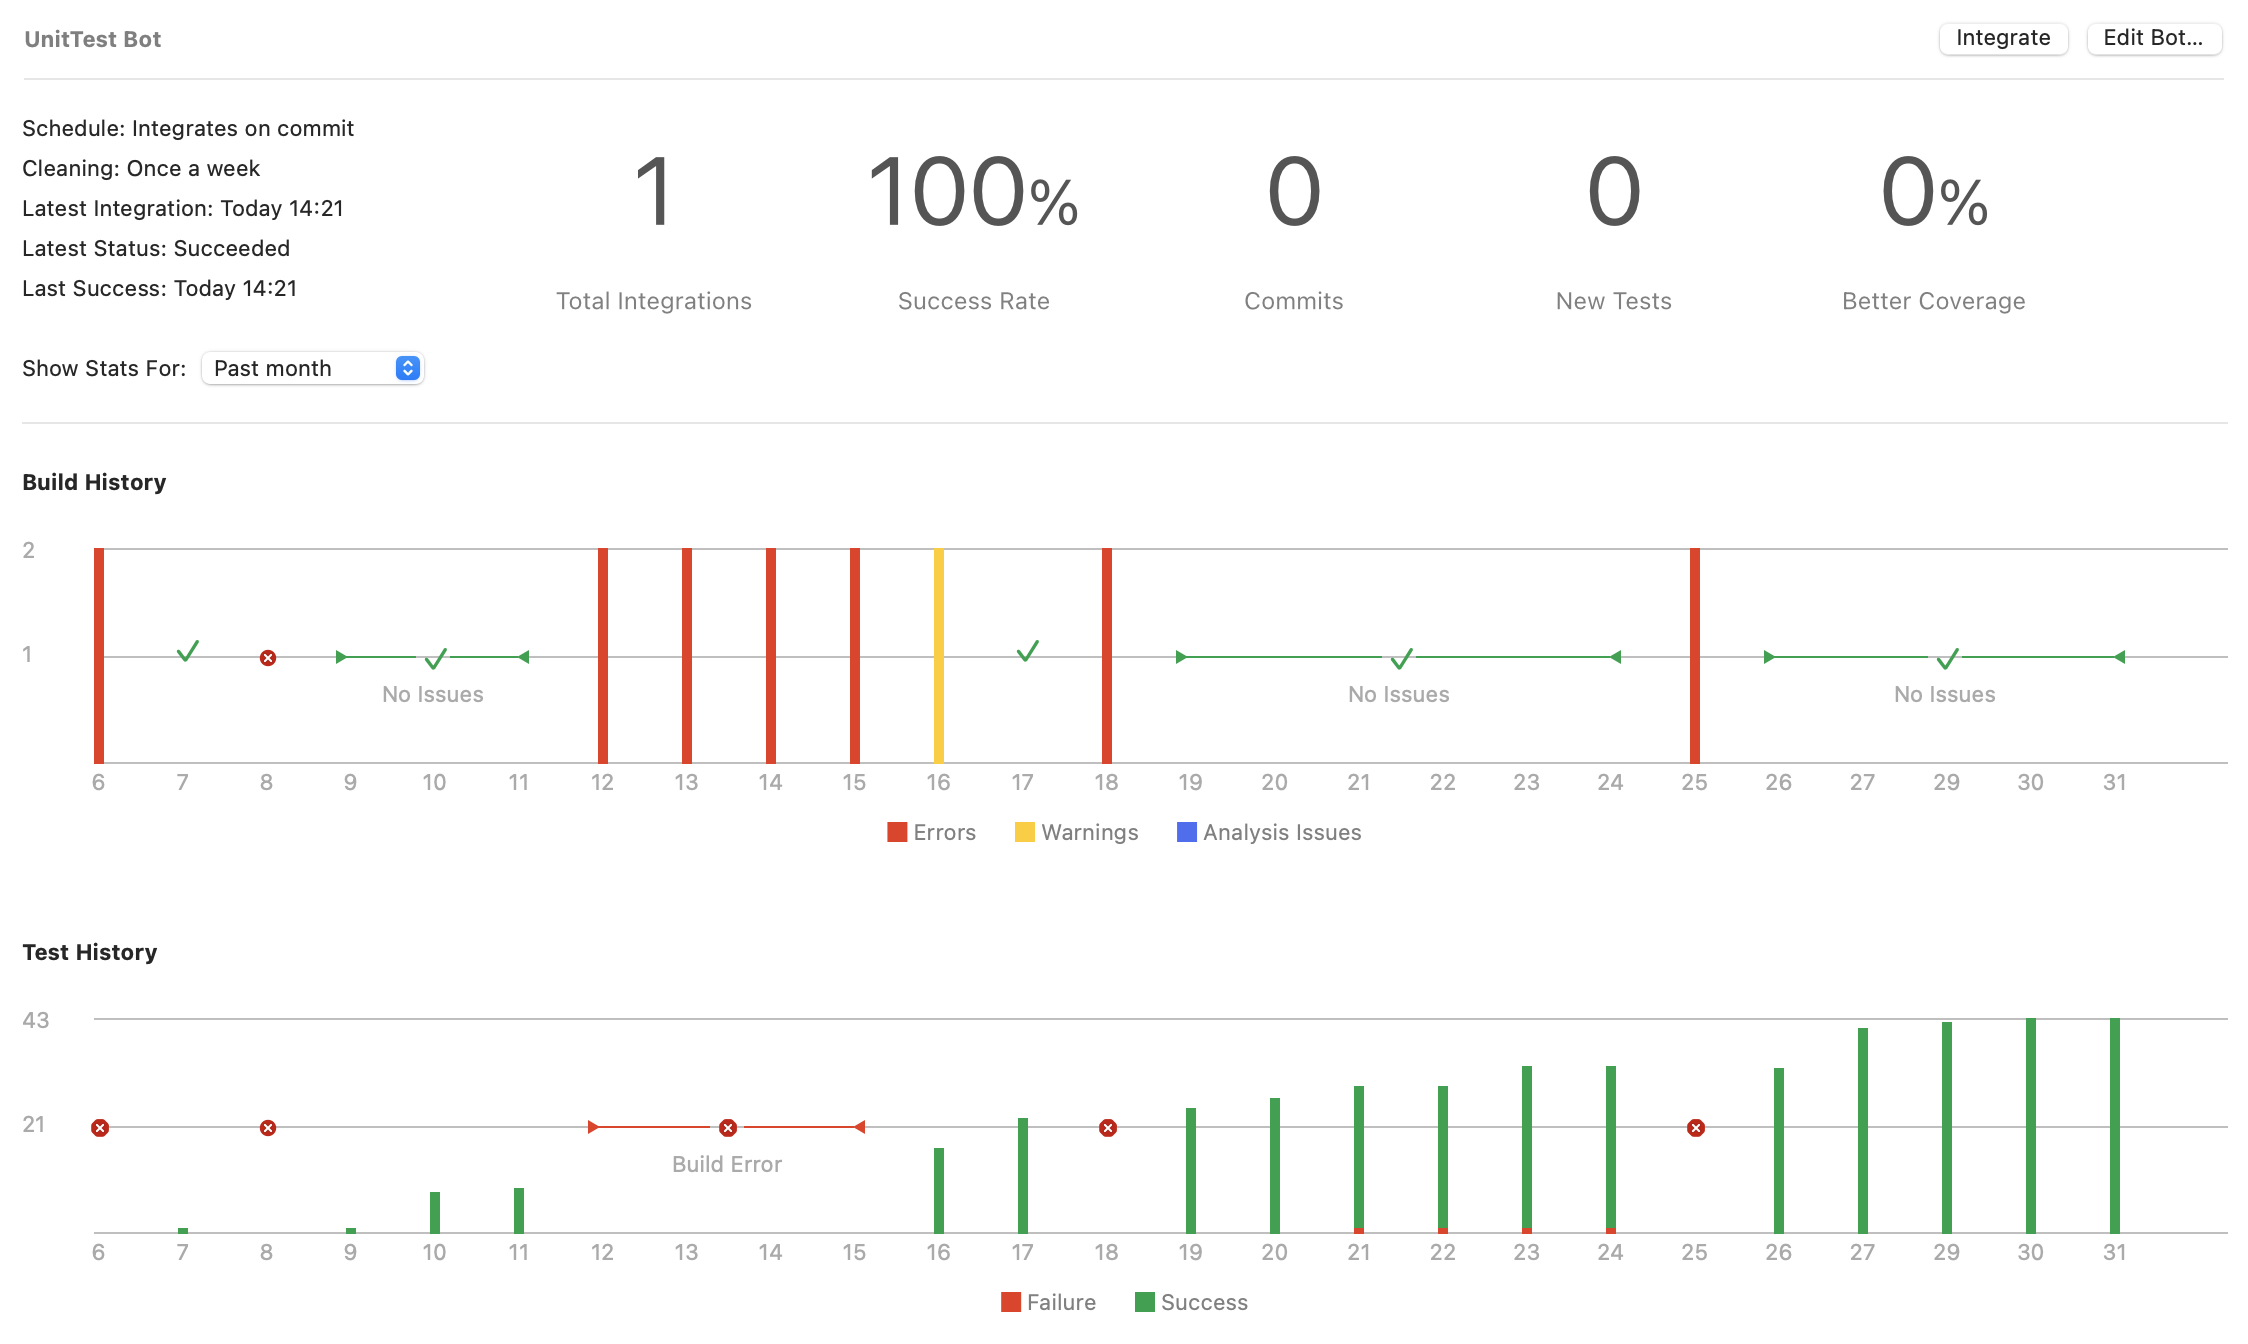
\includegraphics[width=1\textwidth]{img}
  \caption{Painel de integração do \emph{Xcode} \label{fig:int}}
\end{figure}

O \emph{TestBench} e a classe de execução de roteiros foram desenvolvidas com a
interface do \emph{XCTest} em mente e as usam para 
apresentar mensagens de falha quando uma
verificação falha. A Figura~\ref{fig:errmsg} apresenta um exemplo de mensagens de falha
durante a execução de um teste. Na imagem, é possível observar
que, após a subida do \emph{clock} no ciclo oito, o sinal referente ao registrador
$x01$ possuía valor 129 ao invés do esperado de 128, e a falha
foi cascateada em outros erros onde o valor esperado era uma unidade
menor que o valor lido.

\begin{figure}
  \centering
  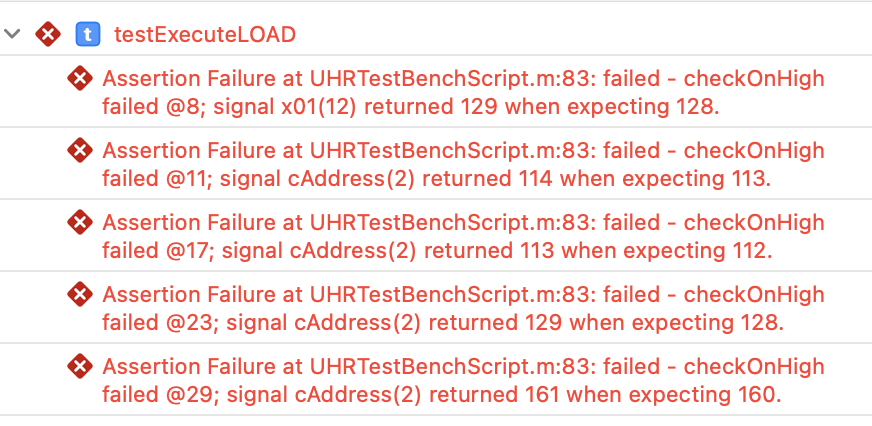
\includegraphics[width=0.5\textwidth]{img2}
  \caption{Exemplo de mensagens de falha de verificação \label{fig:errmsg}}
\end{figure}

\section{Sintetização}
\label{sec:sin}

O processador foi sintetizado para uso em uma placa de desenvolvimento que
utiliza a FPGA \emph{XC7A100T-FGG676ABX1901} da \emph{Xilinx}
e possui o módulo
\emph{CP2102N} da \emph{Silicon Labs} para passar a comunicação UART
através de um cabo USB. A placa também provê um oscilador de cristal
que gera um sinal de \emph{clock} na frequência de 50 \emph{Mhz}, dois botões
e dois diodos emissores de luz.

Para programar a FPGA foi utilizado o \emph{Vivado 2018}, uma suíte
de design da \emph{Xilinx} que possui os programas necessários para
sintetizar a configuração a partir dos módulos e programar o dispositivo.
Além do código em \emph{Verilog}, foi necessário escrever um arquivo
\emph{Xilinx Design Constrain} (XDC) \citep{XDC} que relaciona a entradas e
saídas do módulo de nível mais alto com pinos da FPGA. Com base na folha 
de especificação da placa de desenvolvimento, foi relacionado
quais pinos da \emph{FPGA} representam os dois fios necessários para utilizar o módulo
UART, o gerador de \emph{clock}, os diodos emissores de luz e os botões.
Com base na descrição dos módulos e o arquivo XDC, o \emph{Vivado} gera um arquivo
de configuração. Ao configurar a FPGA com esse arquivo através de uma interface
JTAG, ela passa a funcionar como o processador descrito.


Em relação aos pinos de entrada e saída, o primeiro botão foi mapeado no \emph{bit} 
sB[15][0] e os diodos foram mapeados nos \emph{bits} sB[15][5] e sB[15][4]. Os outros
pinos não foram mapeados em nenhum elemento da placa, e o segundo botão foi mapeado no sinal
de \emph{reset} para inicializar o processador.
Devido a limitação de memória interna da FPGA, foram disponibilizado 
apenas dois bancos de memória para uso na região sD.
\par

%!TeX root=../tese.tex
%("dica" para o editor de texto: este arquivo é parte de um documento maior)
% para saber mais: https://tex.stackexchange.com/q/78101/183146

%% ------------------------------------------------------------------------- %%
\chapter{Conclusão}
\label{cap:4}

\section{Análise de desempenho}
\label{sec:desem}

\section{Considerações sobre o desenvolvimento de processadores RISC-V}
\label{sec:fim}



\par

%\input{conteudo/02...}
%\par

\par


%%%%%%%%%%%%%%%%%%%%%%%%%%%% APÊNDICES E ANEXOS %%%%%%%%%%%%%%%%%%%%%%%%%%%%%%%%

% Um apêndice é algum conteúdo adicional de sua autoria que faz parte e
% colabora com a ideia geral do texto mas que, por alguma razão, não precisa
% fazer parte da sequência do discurso; por exemplo, a demonstração de um
% teorema intermediário, as perguntas usadas em uma pesquisa qualitativa etc.
%
% Um anexo é um documento que não faz parte da tese (em geral, nem é de sua
% autoria) mas é relevante para o conteúdo; por exemplo, a especificação do
% padrão técnico ou a legislação que o trabalho discute, um artigo de jornal
% apresentando a percepção do público sobre o tema da tese etc.
%
% Os comandos appendix e annex reiniciam a numeração de capítulos e passam
% a numerá-los com letras. "annex" não faz parte de nenhuma classe padrão,
% ele foi criado para este modelo (em annex.sty e utils.tex). Se o
% trabalho não tiver apêndices ou anexos, remova estas linhas.
%
% Diferentemente de \mainmatter, \backmatter etc., \appendix e \annex não
% forçam o início de uma nova página. Em geral isso não é importante, pois
% o comando seguinte costuma ser "\chapter", mas pode causar problemas com
% a formatação dos cabeçalhos. Assim, vamos forçar uma nova página antes
% de cada um deles.

%%%% Apêndices %%%%

\makeatletter
\if@openright\cleardoublepage\else\clearpage\fi
\makeatother

\pagestyle{appendix}

\appendix

%!TeX root=../tese.tex
%("dica" para o editor de texto: este arquivo é parte de um documento maior)
% para saber mais: https://tex.stackexchange.com/q/78101/183146

% Apague as duas linhas abaixo (elas servem apenas para gerar um
% aviso no arquivo PDF quando não há nenhum dado a imprimir) e
% insira aqui o conteúdo dos apêndices do seu trabalho (ou deixe
% este arquivo vazio)

%\input{extras/aviso-conteudo}
%\avisoApendices

% Os apêndices podem ser inseridos diretamente aqui ou "puxados" de outros
% arquivos.
% Em alguns (raros) casos, pode ser interessante usar \include ao
% invés de \input: https://tex.stackexchange.com/a/32058/183146

%\input{conteudo/...}
%\par

\par

%%%% Anexos %%%%

\makeatletter
\if@openright\cleardoublepage\else\clearpage\fi
\makeatother

\pagestyle{appendix} % repete o anterior, caso você não use apêndices

\annex

%!TeX root=../tese.tex
%("dica" para o editor de texto: este arquivo é parte de um documento maior)
% para saber mais: https://tex.stackexchange.com/q/78101/183146

% Apague as duas linhas abaixo (elas servem apenas para gerar um
% aviso no arquivo PDF quando não há nenhum dado a imprimir) e
% insira aqui o conteúdo dos anexos do seu trabalho (ou deixe este
% arquivo vazio)

%\input{extras/aviso-conteudo}
%\avisoAnexos

% Os anexos podem ser inseridos diretamente aqui ou "puxados" de outros
% arquivos.
% Em alguns (raros) casos, pode ser interessante usar \include ao
% invés de \input: https://tex.stackexchange.com/a/32058/183146

%\input{conteudo/...}
%\par

\par


%%%%%%%%%%%%%%% SEÇÕES FINAIS (BIBLIOGRAFIA E ÍNDICE REMISSIVO) %%%%%%%%%%%%%%%%

% O comando backmatter desabilita a numeração de capítulos.
\backmatter

\pagestyle{backmatter}

% Espaço adicional no sumário antes das referências / índice remissivo
\addtocontents{toc}{\vspace{2\baselineskip plus .5\baselineskip minus .5\baselineskip}}

% A bibliografia é obrigatória

\printbibliography[
  title=\refname\label{bibliografia}, % "Referências", recomendado pela ABNT
  %title=\bibname\label{bibliografia}, % "Bibliografia"
  heading=bibintoc, % Inclui a bibliografia no sumário
]

\printindex % imprime o índice remissivo no documento (opcional)

\end{document}
